\documentclass[12pt,a4paper]{article}

% ---- Język i kodowanie ----
\usepackage[polish]{babel}
\usepackage[utf8]{inputenc}
\usepackage[T1]{fontenc}
\usepackage{lmodern}
\usepackage{indentfirst}

% ---- Układ strony ----
\usepackage{geometry}
\geometry{margin=2.5cm}
\usepackage{microtype}
\setlength{\parskip}{0.4em}

% ---- Grafika i tabele ----
\usepackage{graphicx}
\usepackage{float}
\usepackage{caption}
\usepackage{subcaption}
\captionsetup{font=small,labelfont=bf}
\usepackage{booktabs}
\usepackage{tabularx}
\usepackage{longtable}
\usepackage{array}
\usepackage{makecell}
\usepackage{multirow}
\usepackage{enumitem}
\setlist{nosep,leftmargin=1.4em}

% ---- Kolory i symbole ----
\usepackage{xcolor}
\definecolor{gold}{HTML}{8A6D3B}
\definecolor{darkgold}{HTML}{5A4A2A}
\definecolor{okgreen}{HTML}{2E7D32}
\usepackage{pifont}
\newcommand{\done}{\textcolor{okgreen}{\ding{51}}}
\newcommand{\na}{\textcolor{gray}{\ding{55}}}

% ---- Listingi / kod ----
\usepackage{listings}
\lstset{
  basicstyle=\ttfamily\small,
  breaklines=true,
  columns=fullflexible,
  keepspaces=true,
  frame=single,
  rulecolor=\color{gold!60},
  backgroundcolor=\color{gold!5},
  literate=%
    {ą}{{\k a}}1 {ć}{{\'c}}1 {ę}{{\k e}}1 {ł}{{\l}}1 {ń}{{\'n}}1
    {ó}{{\'o}}1 {ś}{{\'s}}1 {ż}{{\.z}}1 {ź}{{\'z}}1
    {Ą}{{\k A}}1 {Ć}{{\'C}}1 {Ę}{{\k E}}1 {Ł}{{\L}}1 {Ń}{{\'N}}1
    {Ó}{{\'O}}1 {Ś}{{\'S}}1 {Ż}{{\.Z}}1 {Ź}{{\'Z}}1
}
\newcommand{\code}[1]{\texttt{\detokenize{#1}}}
\usepackage{seqsplit}
\newcommand{\bpath}[1]{\texttt{\expandafter\seqsplit\expandafter{\detokenize{#1}}}}

% ---- Tytuły sekcji ----
\usepackage{titlesec}
\titleformat{\section}{\Large\bfseries\color{darkgold}}{\thesection}{0.6em}{}
\titleformat{\subsection}{\large\bfseries\color{gold}}{\thesubsection}{0.6em}{}

% ---- Hiperłącza ----
\usepackage[hidelinks]{hyperref}
\hypersetup{colorlinks=true,linkcolor=darkgold,urlcolor=gold,citecolor=darkgold}

% ---- Skróty ----
\newcolumntype{Y}{>{\raggedright\arraybackslash}X}
\graphicspath{{obrazy/}{diagramy/}}

\title{
    \large Moduł sumatywny IOAD 2025/2026 \\[0.3em]
    \Huge \textbf{Raport końcowy} \\[0.3em]
    \LARGE Platforma PlayLink \\
    \large \textit{Looking-For-Group dla gier niszowych, retro i mniej popularnych}
}

\author{
    Bartosz Kołaciński, nr indeksu: 251554 \\
    Mateusz Kosowski, nr indeksu: 251558 \\
    Nikodem Nowak, nr indeksu: 251598 \\
    Jakub Rosiak, nr indeksu: 251620 \\
    Jakub Rusek, nr indeksu: 247774 \\[0.6em]
    \normalsize Opiekun projektu: mgr inż. Bartłomiej Jencz
}

\date{\today}

\begin{document}

\maketitle
\begin{center}
\small
Repozytorium: \url{https://github.com/ioad-modul-sumatywny-26/playlink} \\
Demo: \url{https://playlink.bartek.monster} \quad\textbullet\quad
API: \url{https://playlink-backend.bartek.monster/docs}
\end{center}
\newpage

\tableofcontents
\newpage

% =====================================================================
\section{Lista wykonanych punktów}
\label{sec:lista}

Poniższa tabela zestawia wszystkie kryteria oceny modułu sumatywnego ze stanem ich
realizacji w projekcie PlayLink. Symbol \done{} oznacza punkt zrealizowany,
a \na{} — punkt świadomie pominięty (zob.\ przypis).

\renewcommand{\arraystretch}{1.25}
\begin{longtable}{@{}p{0.86\textwidth}c@{}}
\toprule
\textbf{Kryterium} & \textbf{Wyk.} \\
\midrule
\endhead
\multicolumn{2}{@{}l}{\textit{Analiza problemu}} \\
Analiza istniejących rozwiązań (min.\ 3) wraz z oceną zalet i wad (min.\ po 2) & \done \\
Określenie wymagań funkcjonalnych (min.\ 10) & \done \\
Określenie wymagań niefunkcjonalnych (min.\ 5) i ich miar & \done \\
Zidentyfikowanie przypadków użycia wraz ze scenariuszami & \done \\
Diagramy przypadków użycia & \done \\
Wstępna architektura rozwiązania & \done \\
Diagram komponentów & \done \\
Wstępny model rozwiązania (warstwa danych i warstwa logiki) & \done \\
\addlinespace
\multicolumn{2}{@{}l}{\textit{Projekt i implementacja}} \\
Prototyp w wersji podstawowej (min.\ 50\% wymagań funkc.\ i niefunkc.) & \done \\
Prototyp w wersji zaawansowanej (min.\ 70\% wymagań funkc.\ i niefunkc.) & \done \\
Prototyp w wersji zaawansowanej (min.\ 90\% wymagań funkc.\ i niefunkc.) & \done \\
Projekt graficznego interfejsu użytkownika & \done \\
Uwzględnienie wybranych aspektów bezpieczeństwa danych & \done \\
Uwzględnienie co najmniej 90\% aspektów bezpieczeństwa danych & \done \\
\addlinespace
\multicolumn{2}{@{}l}{\textit{Testowanie}} \\
Przeprowadzenie 3 różnych rodzajów testów + dokumentacja & \done \\
Przeprowadzenie 4 różnych rodzajów testów + dokumentacja & \done \\
Przeprowadzenie 5 różnych rodzajów testów + dokumentacja & \done \\
\addlinespace
\multicolumn{2}{@{}l}{\textit{Zarządzanie projektem}} \\
Przygotowanie opisu celów i zakresu projektu & \done \\
Określenie podziału ról i zadań w zespole & \done \\
Sporządzenie raportu końcowego ze wszystkimi wymaganymi elementami & \done \\
Harmonogram realizacji projektu z kamieniami milowymi & \done \\
Szczegółowy harmonogram z kamieniami milowymi i KPI & \done \\
\bottomrule
\end{longtable}
\newpage

% =====================================================================
% =====================================================================
\section{Analiza problemu}
\label{sec:analiza}

\subsection{Pomysł na aplikację}

\textbf{PlayLink} to lekka platforma webowa typu \emph{LFG} (\textit{Looking-For-Group})
służąca do natychmiastowego znajdowania współgraczy do gier niszowych, modów oraz
tytułów retro. Projekt odpowiada na trzy konkretne problemy:

\begin{itemize}
  \item \textbf{Martwe społeczności} — niszowe i stare gry mają zbyt mało aktywnych
        graczy, by samodzielnie utrzymać żywe lobby.
  \item \textbf{Brak dedykowanych narzędzi} — nie istnieje proste narzędzie do szybkiego
        zestawiania partnerów do takich gier.
  \item \textbf{Wysokie bariery wejścia} — istniejące platformy wymagają rejestracji,
        są skomplikowane lub nieaktywne.
\end{itemize}

Odpowiedzią PlayLink jest natychmiastowy dostęp \emph{bez klasycznej rejestracji}
(tożsamość BIP39), przeglądarka aktywnych sesji w czasie rzeczywistym oraz prosty
mechanizm udostępniania pokoju linkiem.

\subsection{Analiza istniejących rozwiązań}
\label{sec:konkurencja}

Przeanalizowano trzy najpopularniejsze alternatywy. Dla każdej wskazano co najmniej
dwie zalety i dwie wady wraz z uzasadnieniem, dlaczego dana cecha jest istotna w
kontekście gier niszowych. Zrzuty ekranu omawianych aplikacji znajdują się w
prezentacji projektowej (załącznik).

\paragraph{Discord — kanały LFG na serwerach.}
Tekstowe kanały „looking-for-group” na serwerach społeczności konkretnych gier, z
komunikacją głosową i tekstową w jednym miejscu.

\begin{itemize}
  \item \textbf{Zalety:}
  \begin{itemize}
    \item Bardzo szybka i bezpośrednia komunikacja (głos + tekst) — kluczowa przy
          umawianiu rozgrywki na żywo.
    \item Ogromna, aktywna baza użytkowników — łatwo znaleźć ludzi do gier popularnych.
  \end{itemize}
  \item \textbf{Wady:}
  \begin{itemize}
    \item Brak dedykowanego systemu sesji — ogłoszenia toną w strumieniu wiadomości i
          szybko znikają, co uniemożliwia ich przeglądanie.
    \item Trzeba znać i dołączyć do konkretnego serwera; brak wyszukiwania ofert
          \emph{między} serwerami — przy grach niszowych właściwe kanały są martwe.
  \end{itemize}
\end{itemize}

\paragraph{Reddit — r/LFG i subreddity gier.}
Tablice ogłoszeń „szukam grupy” w formacie postów na tematycznych subredditach.

\begin{itemize}
  \item \textbf{Zalety:}
  \begin{itemize}
    \item Duża baza użytkowników i prosty, znany format ogłoszeń.
    \item Asynchroniczność — ogłoszenie można zostawić i wrócić do odpowiedzi później.
  \end{itemize}
  \item \textbf{Wady:}
  \begin{itemize}
    \item Całkowity brak komunikacji w czasie rzeczywistym — czeka się na komentarz,
          a posty starzeją się w godzinach, nie w minutach.
    \item Brak filtrowania po grze, regionie czy poziomie oraz brak struktury sesji;
          subreddity gier niszowych są często martwe.
  \end{itemize}
\end{itemize}

\paragraph{FACEIT — matchmaking e-sportowy.}
Profesjonalna platforma e-sportowa z matchmakingiem, ligami i anti-cheatem dla gier
kompetytywnych (CS2, Dota~2, League of Legends).

\begin{itemize}
  \item \textbf{Zalety:}
  \begin{itemize}
    \item Zaawansowany dobór graczy na podstawie umiejętności (skill-based matchmaking).
    \item Duża baza graczy skupionych wokół rywalizacji oraz dedykowane serwery.
  \end{itemize}
  \item \textbf{Wady:}
  \begin{itemize}
    \item Obsługuje wyłącznie popularne tytuły e-sportowe — całkowite pominięcie gier
          niszowych i retro.
    \item Wymaga instalacji klienta i anti-cheata, a część funkcji jest płatna —
          zbyt wysoka bariera dla casualowego gracza.
  \end{itemize}
\end{itemize}

\paragraph{Podsumowanie.}
Żadne z istniejących rozwiązań nie łączy jednocześnie: (1) braku barier wejścia,
(2) struktury sesji z aktualizacją w czasie rzeczywistym oraz (3) wsparcia dla gier
niszowych. PlayLink przejmuje najlepsze elementy konkurencji (czat sesyjny jak na
Discordzie, otwartą listę ogłoszeń jak na Reddicie), eliminuje ich wady (trwała,
przeszukiwalna lista pokojów z filtrowaniem; aktualizacja przez WebSocket) i dodaje
nowe cechy: logowanie bezhasłowe BIP39 oraz kryptograficznie podpisywane wiadomości.

\subsection{Wymagania funkcjonalne}
\label{sec:wf}

Zidentyfikowano 15 wymagań funkcjonalnych; wszystkie zostały zrealizowane w prototypie.

\renewcommand{\arraystretch}{1.25}
\begin{longtable}{@{}clc@{}}
\toprule
\textbf{ID} & \textbf{Wymaganie} & \textbf{Status} \\
\midrule
\endhead
WF-01 & Rejestracja i logowanie bezhasłowe (fraza BIP39 + podpis ECDSA) & \done \\
WF-02 & Odzyskiwanie konta przez import frazy mnemonicznej & \done \\
WF-03 & Edycja nazwy użytkownika (z filtrem wulgaryzmów) & \done \\
WF-04 & Tworzenie i konfiguracja pokoju (gra, limit graczy, lokalizacja) & \done \\
WF-05 & Metadane pokoju (opis, link do komunikatora, wymagania) & \done \\
WF-06 & Przeglądanie listy aktywnych pokojów na żywo & \done \\
WF-07 & Dołączanie do pokoju i jego opuszczanie & \done \\
WF-08 & Czat tekstowy w obrębie pokoju (w czasie rzeczywistym) & \done \\
WF-09 & Kryptograficzne podpisywanie wiadomości czatu (EIP-191) & \done \\
WF-10 & Wyszukiwanie pokojów i użytkowników & \done \\
WF-11 & Filtrowanie pokojów po grze oraz sortowanie listy & \done \\
WF-12 & Kalendarz pokoju i RSVP dla zaplanowanej sesji & \done \\
WF-13 & Własne gry (custom games) i ping zależny od lokalizacji lobby & \done \\
WF-14 & Panel administratora: zarządzanie pokojami i kategoriami gier & \done \\
WF-15 & Moderacja: wyrzucenie uczestnika z pokoju (kick) przez admina & \done \\
\bottomrule
\end{longtable}

\subsection{Wymagania niefunkcjonalne i ich miary}
\label{sec:wnf}

\renewcommand{\arraystretch}{1.3}
\begin{longtable}{@{}cp{0.30\textwidth}p{0.46\textwidth}c@{}}
\toprule
\textbf{ID} & \textbf{Wymaganie} & \textbf{Miara / kryterium akceptacji} & \textbf{St.} \\
\midrule
\endhead
WN-01 & Wydajność & Czas odpowiedzi API $<$ 200~ms dla 95\% żądań (p95) & \done \\
WN-02 & Responsywność realtime & Aktualizacja UI po zdarzeniu $<$ 1000~ms & \done \\
WN-03 & Dostępność & Uptime $\geq$ 99\% w skali miesiąca & \done \\
WN-04 & Skalowalność & Do 128 użytkowników jednocześnie w pokoju & \done \\
WN-05 & Niezawodność & Docker healthcheck + automatyczny restart kontenera & \done \\
WN-06 & Realtime / odporność & WebSocket z heartbeatem 30~s i auto-reconnectem & \done \\
WN-07 & Bezpieczeństwo transportu & TLS~1.3 dla HTTPS i WSS (Let's Encrypt) & \done \\
WN-08 & Ochrona przed nadużyciami & Rate limiting: 10/min (REST), 10~wiad./10~s (czat WS) & \done \\
WN-09 & Użyteczność & Utworzenie pokoju w $\leq$ 30~s bez instrukcji & \done \\
WN-10 & Modułowość & Frontend i backend wdrażane niezależnie & \done \\
WN-11 & Jakość kodu & Pokrycie testami backendu $\geq$ 80\% (bramka CI) & \done \\
WN-12 & Wdrażalność & Czas od \code{push} do wersji live $\approx$ 3~min & \done \\
\bottomrule
\end{longtable}

\subsection{Przypadki użycia i scenariusze}
\label{sec:uc}

W systemie występują czterej aktorzy: \textbf{Gość} (niezalogowany), \textbf{Użytkownik}
(zalogowany, dziedziczy uprawnienia Gościa), \textbf{Administrator} (dziedziczy
uprawnienia Użytkownika) oraz \textbf{System} (zadania automatyczne — weryfikacja
challenge-response i czyszczenie wygasłych pokojów).

\paragraph{Lista przypadków użycia.}
\begin{itemize}
  \item \textbf{Gość:} przeglądanie listy pokojów; wyszukiwanie i filtrowanie;
        rejestracja / logowanie.
  \item \textbf{Użytkownik:} tworzenie i konfiguracja pokoju; dołączanie/opuszczanie;
        czat (podpisany); planowanie wydarzenia i RSVP; edycja nazwy; odzyskiwanie konta.
  \item \textbf{Administrator:} wyrzucenie uczestnika (kick); zarządzanie kategoriami gier.
  \item \textbf{System:} weryfikacja podpisu i wydanie JWT; czyszczenie wygasłych
        pokojów i wiadomości.
\end{itemize}

Diagram przypadków użycia przedstawiono na rys.~\ref{fig:uc}. Poniżej opisano
scenariusze pięciu kluczowych przypadków użycia — po jednym opracowanym przez
każdego członka zespołu — w ujęciu: przepływ główny oraz przepływ alternatywny.

\paragraph{UC-1: Rejestracja i pierwsze logowanie (BIP39). \normalfont\textit{(autor: Nikodem Nowak)}}
\begin{itemize}
  \item \textit{Aktor:} Gość. \quad \textit{Warunek wstępny:} brak.
  \item \textit{Przepływ główny:}
  \begin{enumerate}
    \item Gość wybiera „Enter realm” i generuje nową 12-słowną frazę BIP39
          (klucz prywatny derywowany lokalnie, nigdy nie opuszcza przeglądarki).
    \item Klient pobiera z backendu jednorazowy \emph{nonce} (\code{POST /auth/request-nonce}).
    \item Klient podpisuje komunikat zawierający nonce (\code{personal_sign}, EIP-191).
    \item Backend odtwarza adres z podpisu, weryfikuje nonce i wydaje token JWT
          (\code{POST /auth/verify}).
    \item BFF zapisuje JWT w ciasteczku \code{httpOnly}; użytkownik jest zalogowany.
  \end{enumerate}
  \item \textit{Przepływ alternatywny:} nonce wygasł lub został już użyty —
        backend odrzuca weryfikację (HTTP 400/401), klient ponawia od kroku~2.
\end{itemize}

\paragraph{UC-2: Utworzenie pokoju i rozpoczęcie czatu. \normalfont\textit{(autor: Bartosz Kołaciński)}}
\begin{itemize}
  \item \textit{Aktor:} Użytkownik. \quad \textit{Warunek wstępny:} zalogowany; mniej niż
        3 aktywne pokoje.
  \item \textit{Przepływ główny:}
  \begin{enumerate}
    \item Użytkownik wypełnia formularz (nazwa, gra, limit graczy, lokalizacja,
          opcjonalnie opis/link/wymagania) i zatwierdza.
    \item Backend tworzy pokój, dołącza twórcę jako członka i rozgłasza nową listę
          pokojów przez kanał \code{/ws/rooms}.
    \item Użytkownik wchodzi do pokoju; otwiera się kanał czatu
          \code{/ws/rooms/<name>/chat}.
  \end{enumerate}
  \item \textit{Przepływ alternatywny:} przekroczony limit 3 pokojów lub zajęta nazwa —
        backend zwraca błąd walidacji, formularz wyświetla komunikat.
\end{itemize}

\paragraph{UC-3: Dołączenie do pokoju i deklaracja RSVP. \normalfont\textit{(autor: Jakub Rosiak)}}
\begin{itemize}
  \item \textit{Aktor:} Użytkownik. \quad \textit{Warunek wstępny:} pokój istnieje i nie
        jest pełny.
  \item \textit{Przepływ główny:}
  \begin{enumerate}
    \item Użytkownik wybiera pokój z listy i dołącza; roster jest rozgłaszany do
          pozostałych członków.
    \item Jeśli pokój ma zaplanowane wydarzenie, użytkownik deklaruje obecność
          (\emph{present} / \emph{maybe} / \emph{absent}); zdarzenie RSVP jest rozgłaszane.
    \item Użytkownik bierze udział w czacie pokoju.
  \end{enumerate}
  \item \textit{Przepływ alternatywny:} pokój pełny lub wygasł — dołączenie zostaje
        odrzucone, użytkownik wraca do listy.
\end{itemize}

\paragraph{UC-4: Moderacja — wyrzucenie uczestnika. \normalfont\textit{(autor: Jakub Rusek)}}
\begin{itemize}
  \item \textit{Aktor:} Administrator. \quad \textit{Warunek wstępny:} adres administratora
        znajduje się w \code{ADMIN_ADDRESSES}.
  \item \textit{Przepływ główny:}
  \begin{enumerate}
    \item Administrator wybiera uczestnika i akcję „kick”.
    \item Backend weryfikuje uprawnienia, usuwa członkostwo i rozgłasza ramkę
          \emph{kick} oraz zaktualizowany roster; wyrzucony klient zostaje rozłączony.
  \end{enumerate}
  \item \textit{Przepływ alternatywny:} żądanie pochodzi od konta bez uprawnień
        administratora — backend odrzuca operację (HTTP 403).
\end{itemize}

\paragraph{UC-5: Wyszukiwanie i filtrowanie pokojów. \normalfont\textit{(autor: Mateusz Kosowski)}}
\begin{itemize}
  \item \textit{Aktor:} Gość lub Użytkownik. \quad \textit{Warunek wstępny:} brak.
  \item \textit{Przepływ główny:}
  \begin{enumerate}
    \item Aktor otwiera listę pokojów, która jest na bieżąco aktualizowana przez
          kanał \code{/ws/rooms}.
    \item Aktor wpisuje frazę wyszukiwania i/lub wybiera filtr gry oraz porządek
          sortowania.
    \item Lista zawęża się do pokojów spełniających kryteria; wybór pokoju prowadzi
          do jego szczegółów (a po zalogowaniu — do dołączenia, UC-2/UC-3).
  \end{enumerate}
  \item \textit{Przepływ alternatywny:} brak pokojów spełniających kryteria —
        wyświetlany jest stan pusty z podpowiedzią rozszerzenia filtrów lub utworzenia
        własnego pokoju.
\end{itemize}

\subsection{Diagram przypadków użycia}
\label{sec:uc-diagram}

\begin{figure}[H]
  \centering
  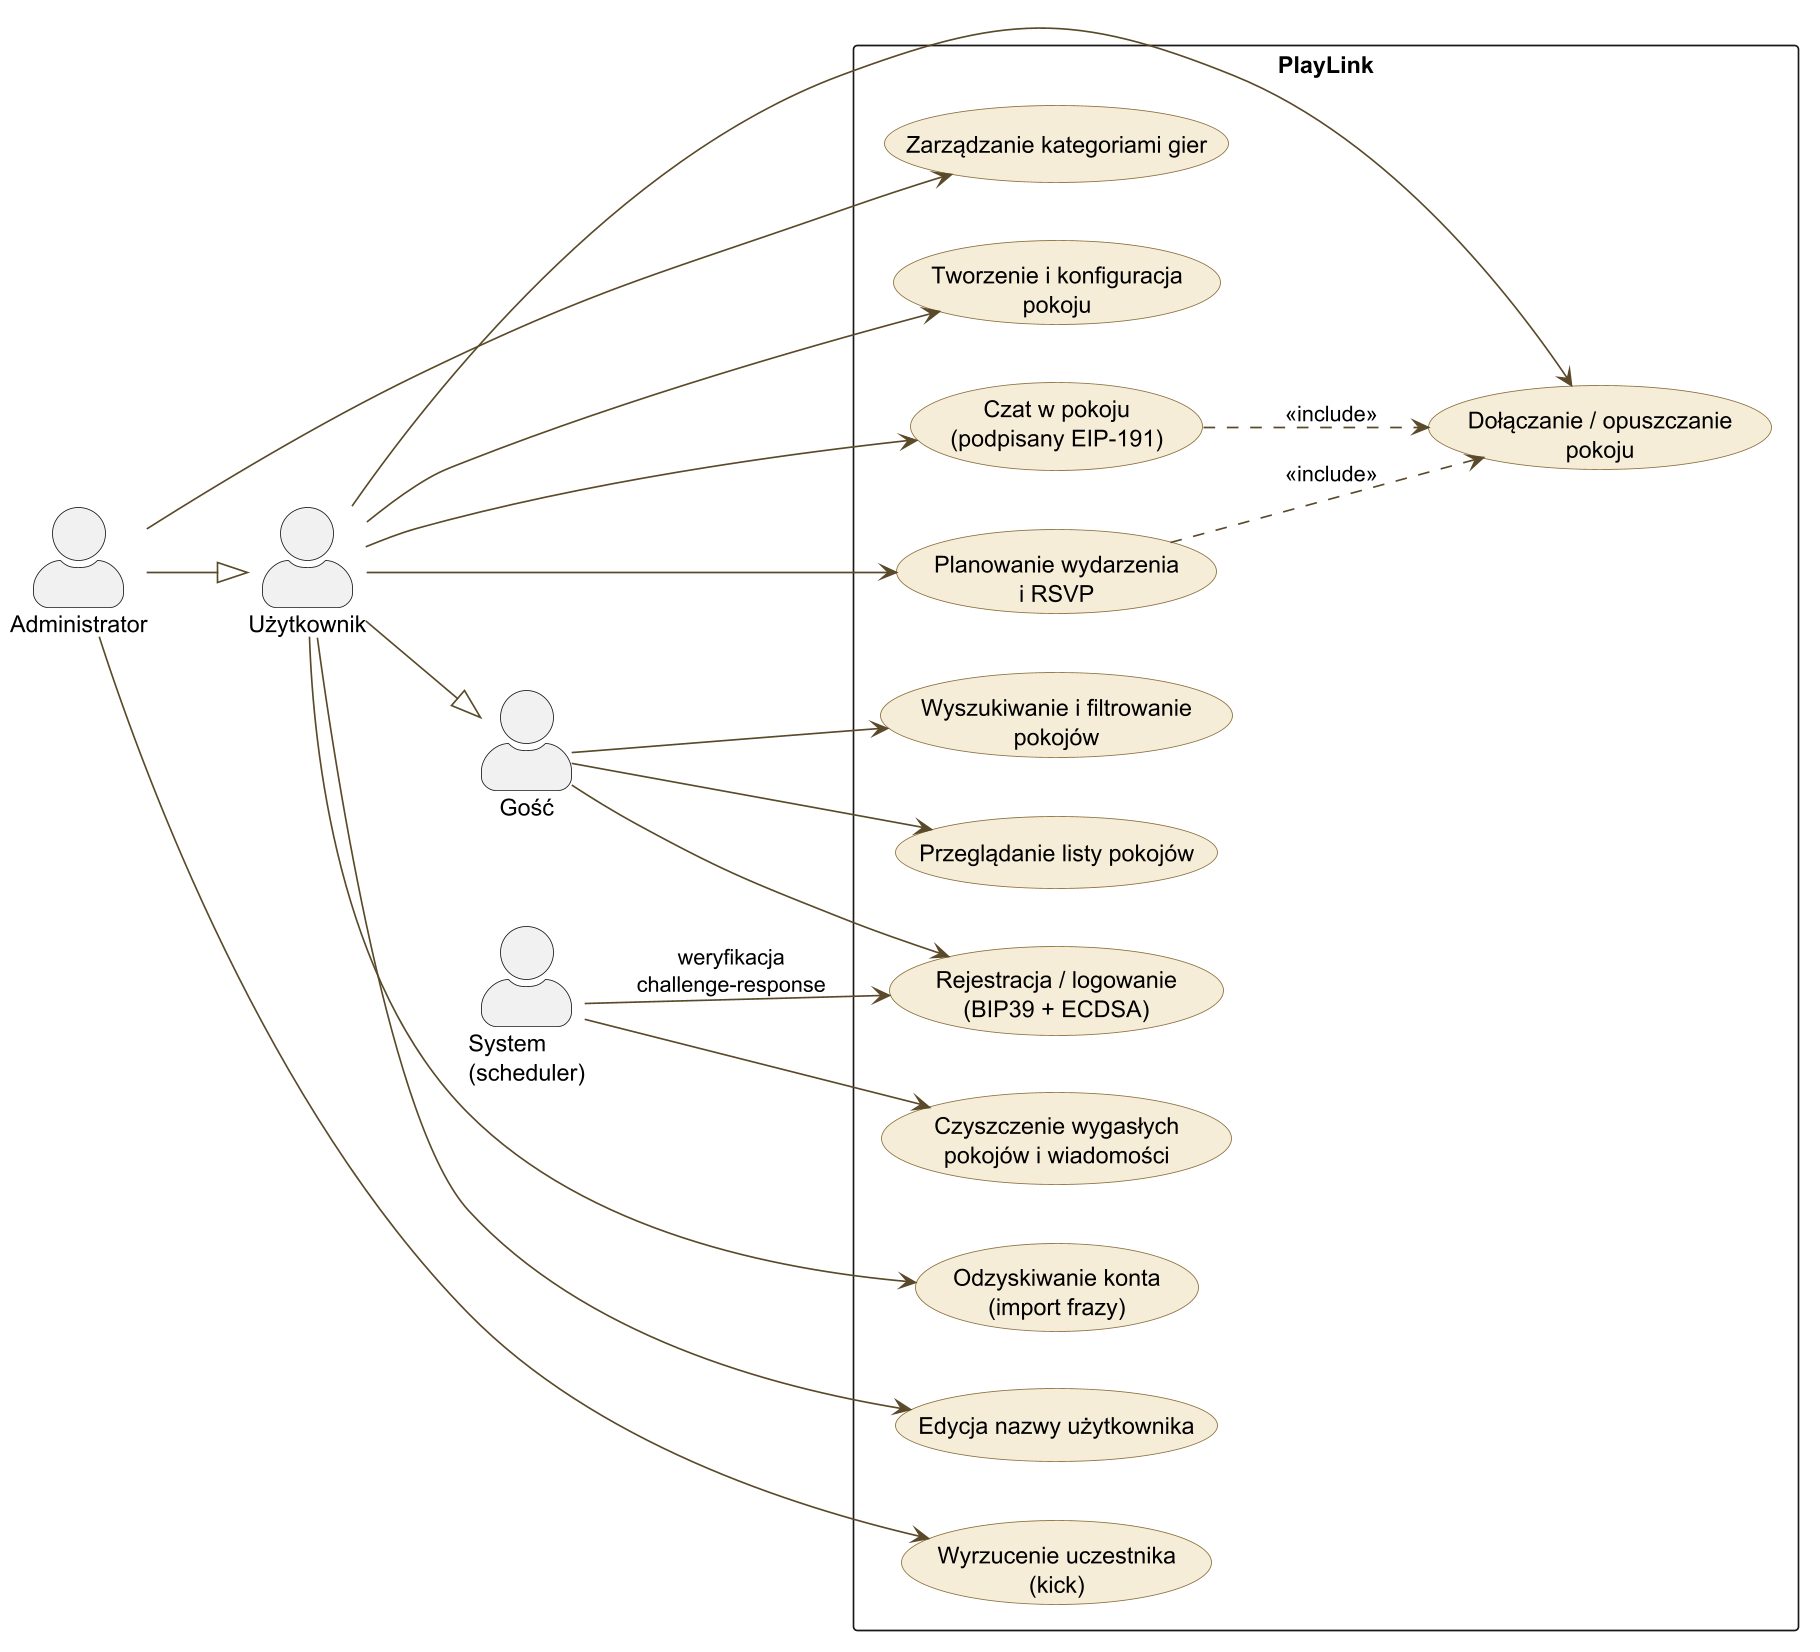
\includegraphics[width=0.95\textwidth]{uc.png}
  \caption{Diagram przypadków użycia PlayLink (aktorzy: Gość, Użytkownik,
  Administrator, System).}
  \label{fig:uc}
\end{figure}

\subsection{Wstępna architektura rozwiązania}
\label{sec:architektura}

PlayLink ma architekturę trójwarstwową z wzorcem \textbf{BFF}
(\textit{Backend-for-Frontend}). Przeglądarka komunikuje się \emph{bezpośrednio} z
API (REST oraz dwa kanały WebSocket) dla większości odczytów i całego ruchu realtime,
a z serwerem SvelteKit (BFF) tylko dla operacji wymagających dostępu do ciasteczka
sesyjnego \code{httpOnly} (logowanie/wylogowanie oraz uwierzytelnione akcje formularzy),
które BFF proxy-uje do backendu z dołączonym tokenem JWT.

\begin{itemize}
  \item \textbf{Wzorce projektowe:} BFF (izolacja JWT od JavaScriptu klienta),
        wstrzykiwanie zależności (FastAPI \code{Depends}), wzorzec repozytorium przez
        SQLModel/SQLAlchemy, publish–subscribe dla rozgłaszania zdarzeń WebSocket.
  \item \textbf{Główne moduły:} klient Svelte (podpisywanie BIP39 przez ethers/viem),
        BFF SvelteKit (adapter-node), API FastAPI (REST + WebSocket + zadanie w tle),
        baza PostgreSQL.
  \item \textbf{Stos technologiczny} zestawiono w tab.~\ref{tab:stack}.
\end{itemize}

\renewcommand{\arraystretch}{1.2}
\begin{table}[H]
\centering\small
\begin{tabularx}{\textwidth}{@{}lY@{}}
\toprule
\textbf{Warstwa} & \textbf{Technologia} \\
\midrule
Frontend & SvelteKit~2 / Svelte~5 (runes), TypeScript, Tailwind CSS (build: Bun) \\
Podpisywanie & ethers + viem (BIP39 + EIP-191) \\
Backend & FastAPI (Python 3.14+), serwer ASGI (build: uv) \\
ORM / migracje & SQLModel (SQLAlchemy + Pydantic), Alembic \\
Baza danych & PostgreSQL~18 (prod) / SQLite in-memory (testy) \\
Realtime & FastAPI WebSockets (kanały: rooms, chat) \\
Uwierzytelnianie & tożsamość BIP39 + ECDSA (\code{eth_account}), JWT HS256 \\
Rate limiting & slowapi (REST) + przesuwne okno per-adres (czat) \\
Orkiestracja & Docker Compose (db, backend, frontend), Nginx, Tailscale \\
CI/CD & GitHub Actions $\rightarrow$ deploy SSH przez Tailscale \\
\bottomrule
\end{tabularx}
\caption{Stos technologiczny PlayLink.}
\label{tab:stack}
\end{table}

Przepływ uwierzytelniania challenge-response przedstawia rys.~\ref{fig:auth}.

\begin{figure}[H]
  \centering
  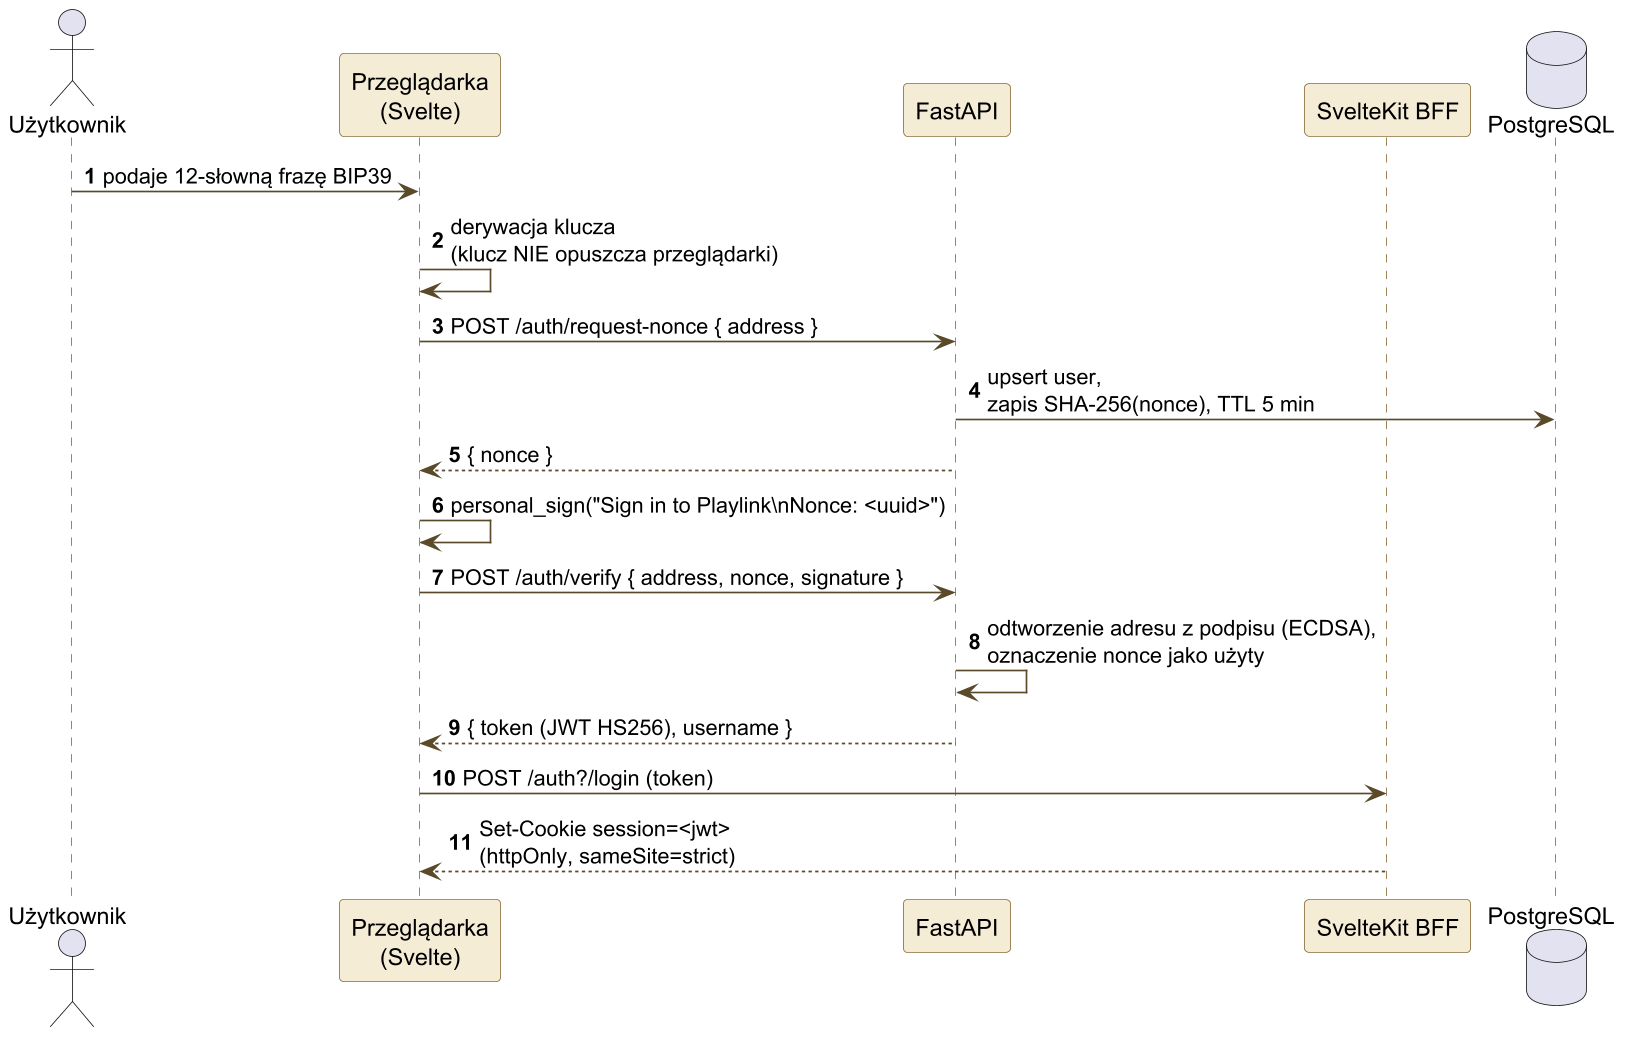
\includegraphics[width=0.92\textwidth]{sekwencja-auth.png}
  \caption{Diagram sekwencji: bezhasłowe logowanie (challenge-response BIP39/ECDSA).
  Klucz prywatny nigdy nie opuszcza przeglądarki; JWT trafia do ciasteczka
  \texttt{httpOnly} ustawianego przez BFF.}
  \label{fig:auth}
\end{figure}

\subsection{Diagram komponentów}
\label{sec:komponenty}

\begin{figure}[H]
  \centering
  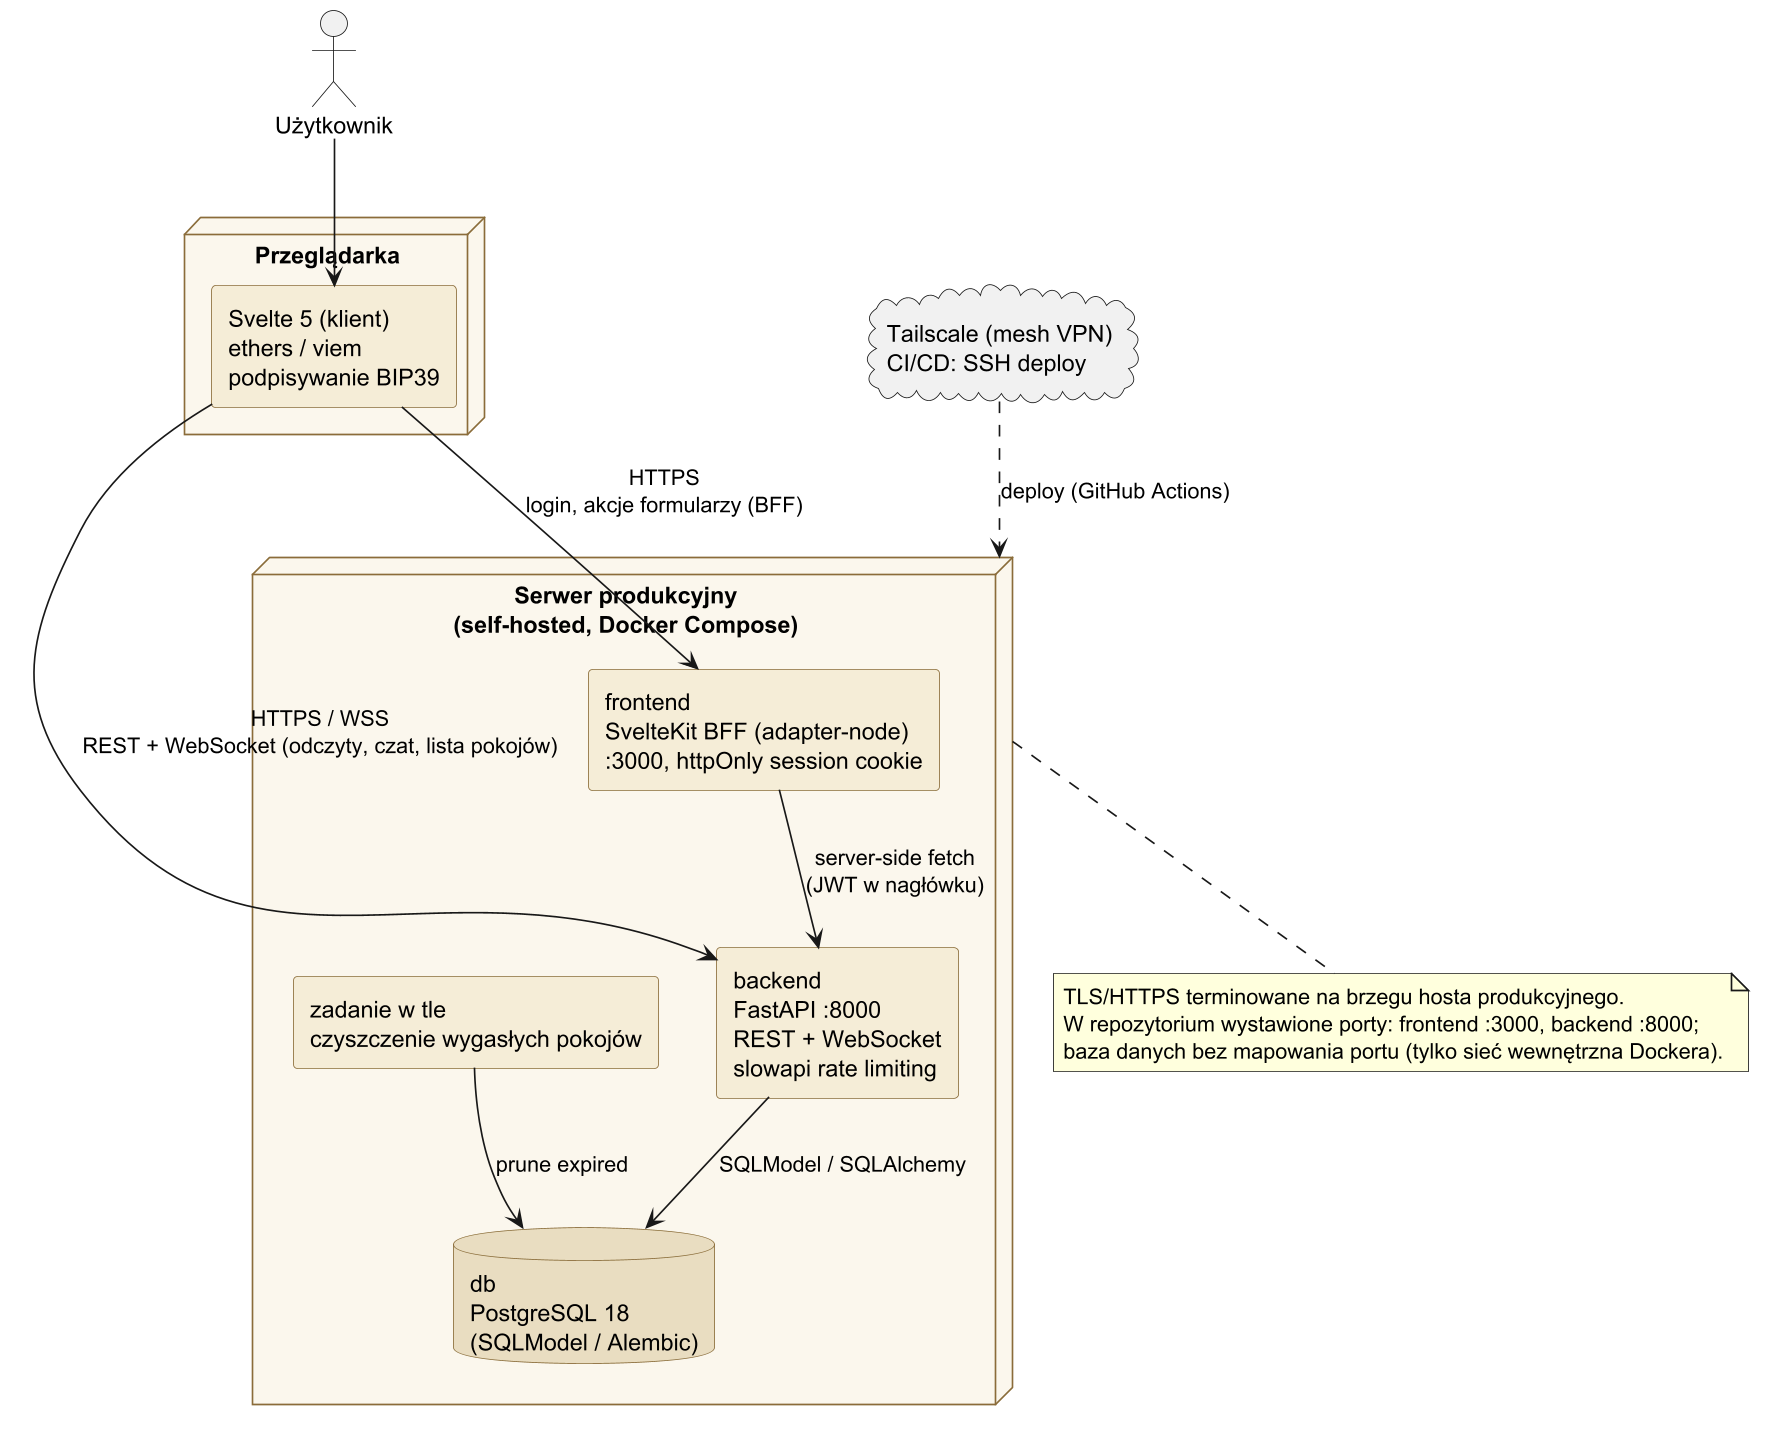
\includegraphics[width=0.85\textwidth]{komponenty.png}
  \caption{Diagram komponentów: przeglądarka, Nginx (TLS), BFF SvelteKit, API FastAPI
  z zadaniem czyszczącym oraz baza PostgreSQL; wdrożenie przez Tailscale.}
  \label{fig:komponenty}
\end{figure}

\subsection{Wstępny model rozwiązania: warstwa danych i warstwa logiki}
\label{sec:model}

\subsubsection*{Warstwa danych}

Trwałość zapewnia PostgreSQL z ośmioma encjami zarządzanymi przez SQLModel i migracjami
Alembic. Model danych przedstawia diagram ERD na rys.~\ref{fig:er}.

\begin{itemize}
  \item \code{user} — tożsamość: \code{identity_address} (adres EIP-55 odtworzony z ECDSA)
        oraz unikalna \code{username}; \emph{brak hasła}.
  \item \code{nonce} — jednorazowe, krótkożyciowe wyzwania; w bazie przechowywany jest
        wyłącznie skrót SHA-256 wartości nonce (\code{value}), z flagą \code{used}.
  \item \code{room} — sesja gry: nazwa (unikalna), gra, lokalizacja lobby, limit graczy,
        metadane oraz \code{expires_at} (TTL, domyślnie 60~min).
  \item \code{roommember} — tabela łącząca (M:N) użytkowników i pokoje (klucz złożony).
  \item \code{message} — wiadomości czatu; opcjonalny podpis EIP-191 (\code{signature})
        i podpisany znacznik czasu (\code{sent_at}) zapewniają weryfikowalne autorstwo.
  \item \code{roomevent} / \code{roomeventrsvp} — zaplanowane wydarzenie pokoju oraz
        deklaracje obecności (status \emph{present}/\emph{absent}/\emph{maybe},
        semantyka upsert).
  \item \code{game} — katalog kategorii gier (kolejność wg \code{sort_order}).
\end{itemize}

\begin{figure}[H]
  \centering
  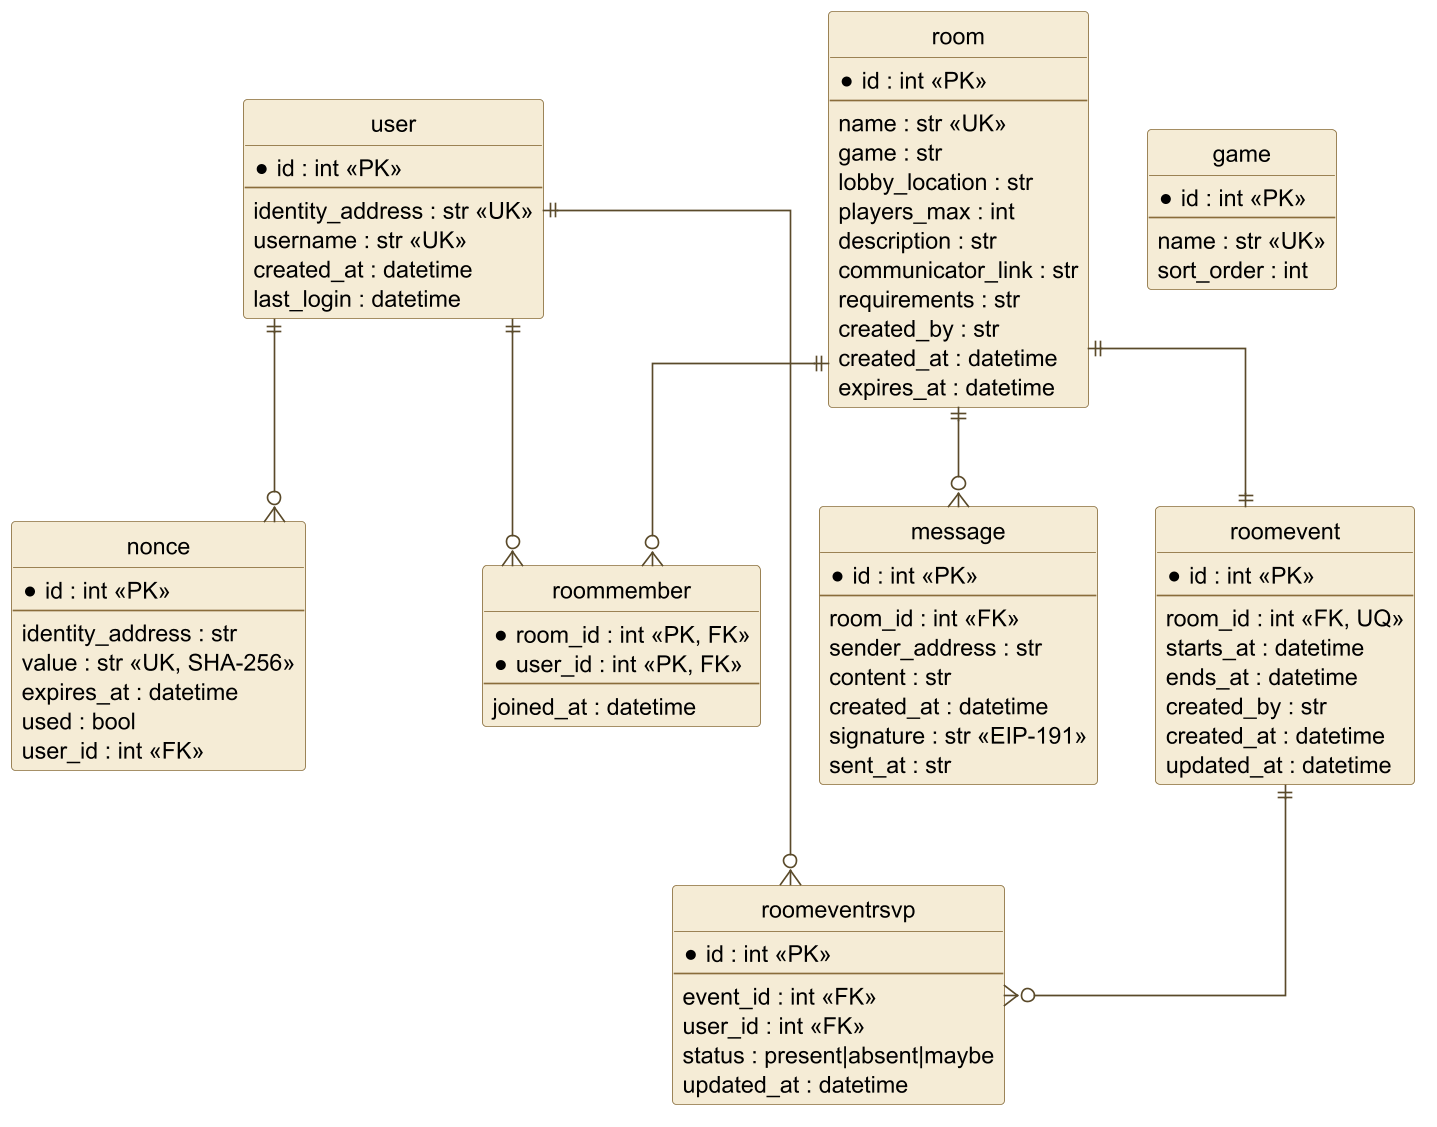
\includegraphics[width=\textwidth]{er.png}
  \caption{Model danych (ERD) PlayLink — osiem encji wraz z kluczami i relacjami.}
  \label{fig:er}
\end{figure}

\subsubsection*{Warstwa logiki}

Logika backendu jest skupiona w usłudze FastAPI udostępniającej REST oraz dwa kanały
WebSocket. Najważniejsze elementy:

\begin{itemize}
  \item \textbf{REST} — endpointy uwierzytelniania (\code{/auth/request-nonce},
        \code{/auth/verify}), CRUD pokojów, profil użytkownika, administracja.
        Dokumentacja generowana automatycznie (Swagger/OpenAPI).
  \item \textbf{WebSocket} — kanał \code{/ws/rooms} (rozgłasza pełną listę pokojów po
        każdej mutacji) oraz \code{/ws/rooms/<name>/chat} (czat z autoryzacją JWT i
        kontrolą członkostwa; ramki: event, RSVP, roster, room-closed, kick).
  \item \textbf{Logika biznesowa} — m.in.: limit 3 aktywnych pokojów na użytkownika,
        weryfikacja podpisów EIP-191 z odrzuceniem nadmiernego dryfu czasu
        (\code{CHAT_SIGNATURE_SKEW_SECONDS}), upsert RSVP, dobór pingu na podstawie
        lokalizacji lobby (odległość Haversine).
  \item \textbf{Zadanie w tle} — cykliczne czyszczenie wygasłych pokojów i wiadomości
        (co \code{ROOM_CLEANUP_INTERVAL_SECONDS}).
\end{itemize}

% =====================================================================
\section{Projekt i implementacja rozwiązania}
\label{sec:impl}

\subsection{Stopień realizacji wymagań}

Prototyp PlayLink osiągnął poziom \textbf{wersji zaawansowanej ($\geq$90\%)}. Wszystkie
15 wymagań funkcjonalnych z tab.~\ref{sec:wf} oraz wszystkie 12 wymagań niefunkcjonalnych
z tab.~\ref{sec:wnf} zostały zrealizowane i wdrożone na środowisku produkcyjnym
(\url{https://playlink.bartek.monster}). Aplikacja jest w pełni działająca:
uwierzytelnianie BIP39, tworzenie/dołączanie/opuszczanie pokojów, czat realtime z
podpisami, kalendarz i RSVP, wyszukiwanie i filtrowanie, panel administratora oraz
automatyczne czyszczenie wygasłych pokojów.

Zastosowano aktualne standardy projektowe: typowanie statyczne w całym stosie
(TypeScript + Pydantic/SQLModel), automatyczną walidację żądań, migracje bazy
(Alembic) oraz w pełni zautomatyzowany pipeline CI/CD (rozdz.~\ref{sec:zarz}).

\subsection{Projekt graficznego interfejsu użytkownika}
\label{sec:gui}

Interfejs zaprojektowano w estetyce inspirowanej przeglądarką lobby z gry
\textit{Diablo~II: Resurrected} — ciemna, gotycka paleta złoto-brązowa i
minimalistyczny układ. Frontend zbudowano w SvelteKit~2 / Svelte~5 (runes) z Tailwind
CSS; UI reaguje natychmiast na zdarzenia WebSocket. Poniżej wybrane widoki aplikacji.

\begin{figure}[H]
  \centering
  \begin{subfigure}[t]{0.48\textwidth}
    
\includegraphics[width=\textwidth]{prez-slide25.png}
    \caption{Strona startowa („Enter realm”).}
  \end{subfigure}\hfill
  \begin{subfigure}[t]{0.48\textwidth}
    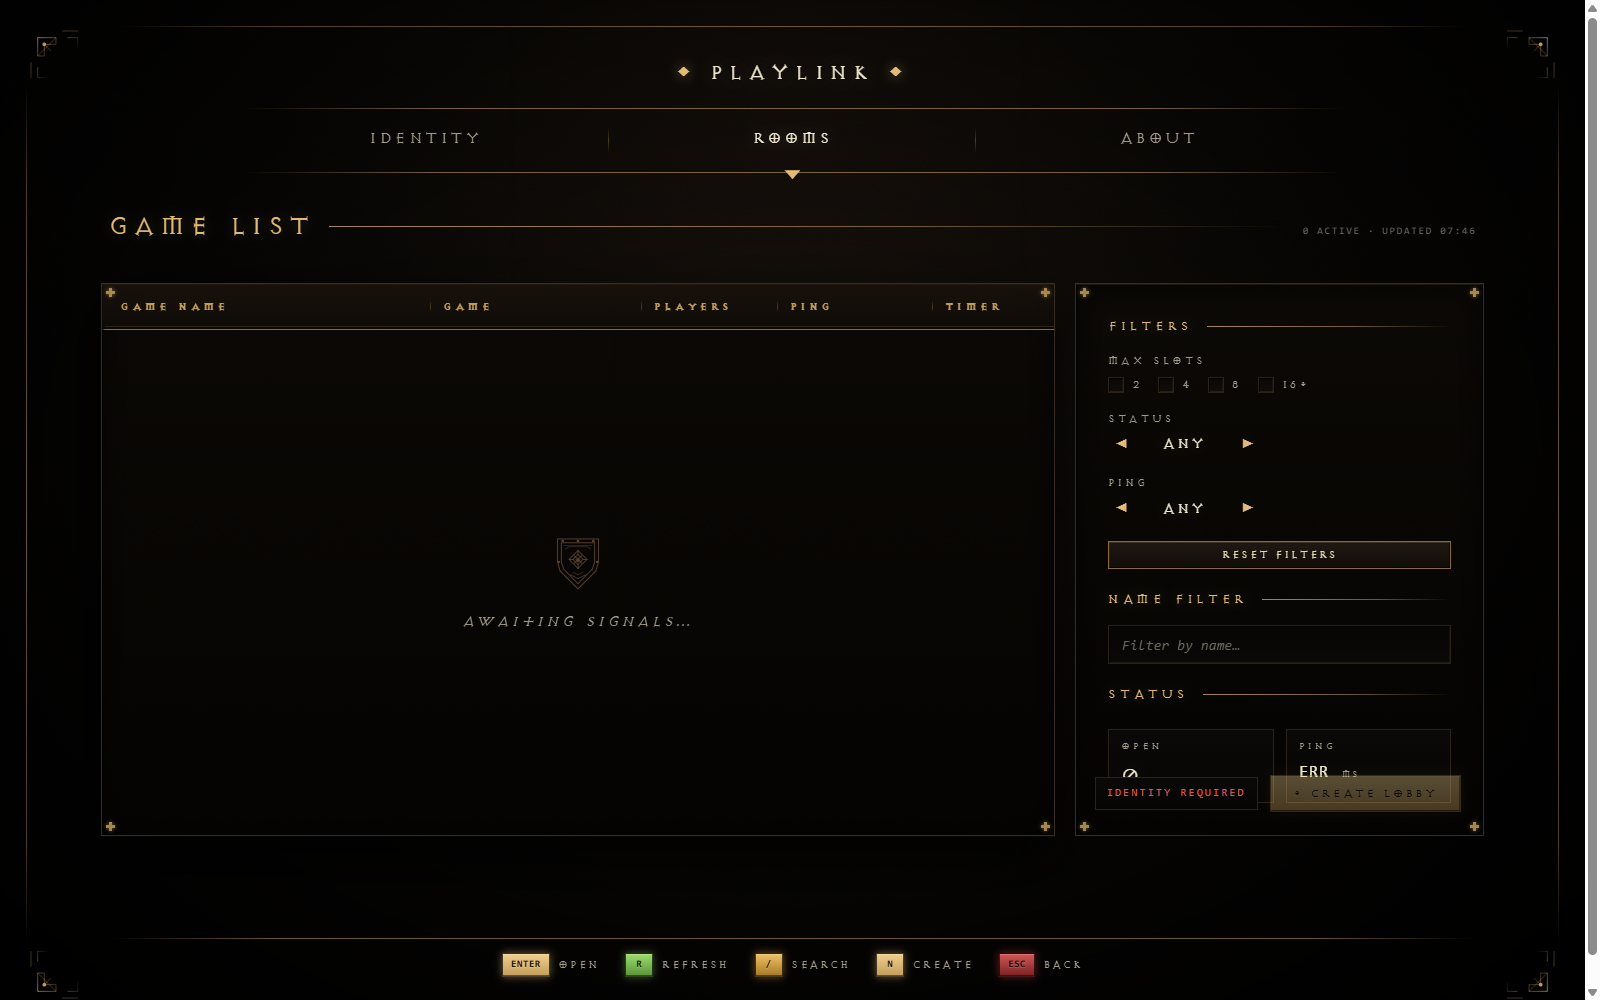
\includegraphics[width=\textwidth]{d2-rooms-v1.png}
    \caption{Przeglądarka pokojów (lista lobby).}
  \end{subfigure}

  \vspace{0.7em}
  \begin{subfigure}[t]{0.48\textwidth}
    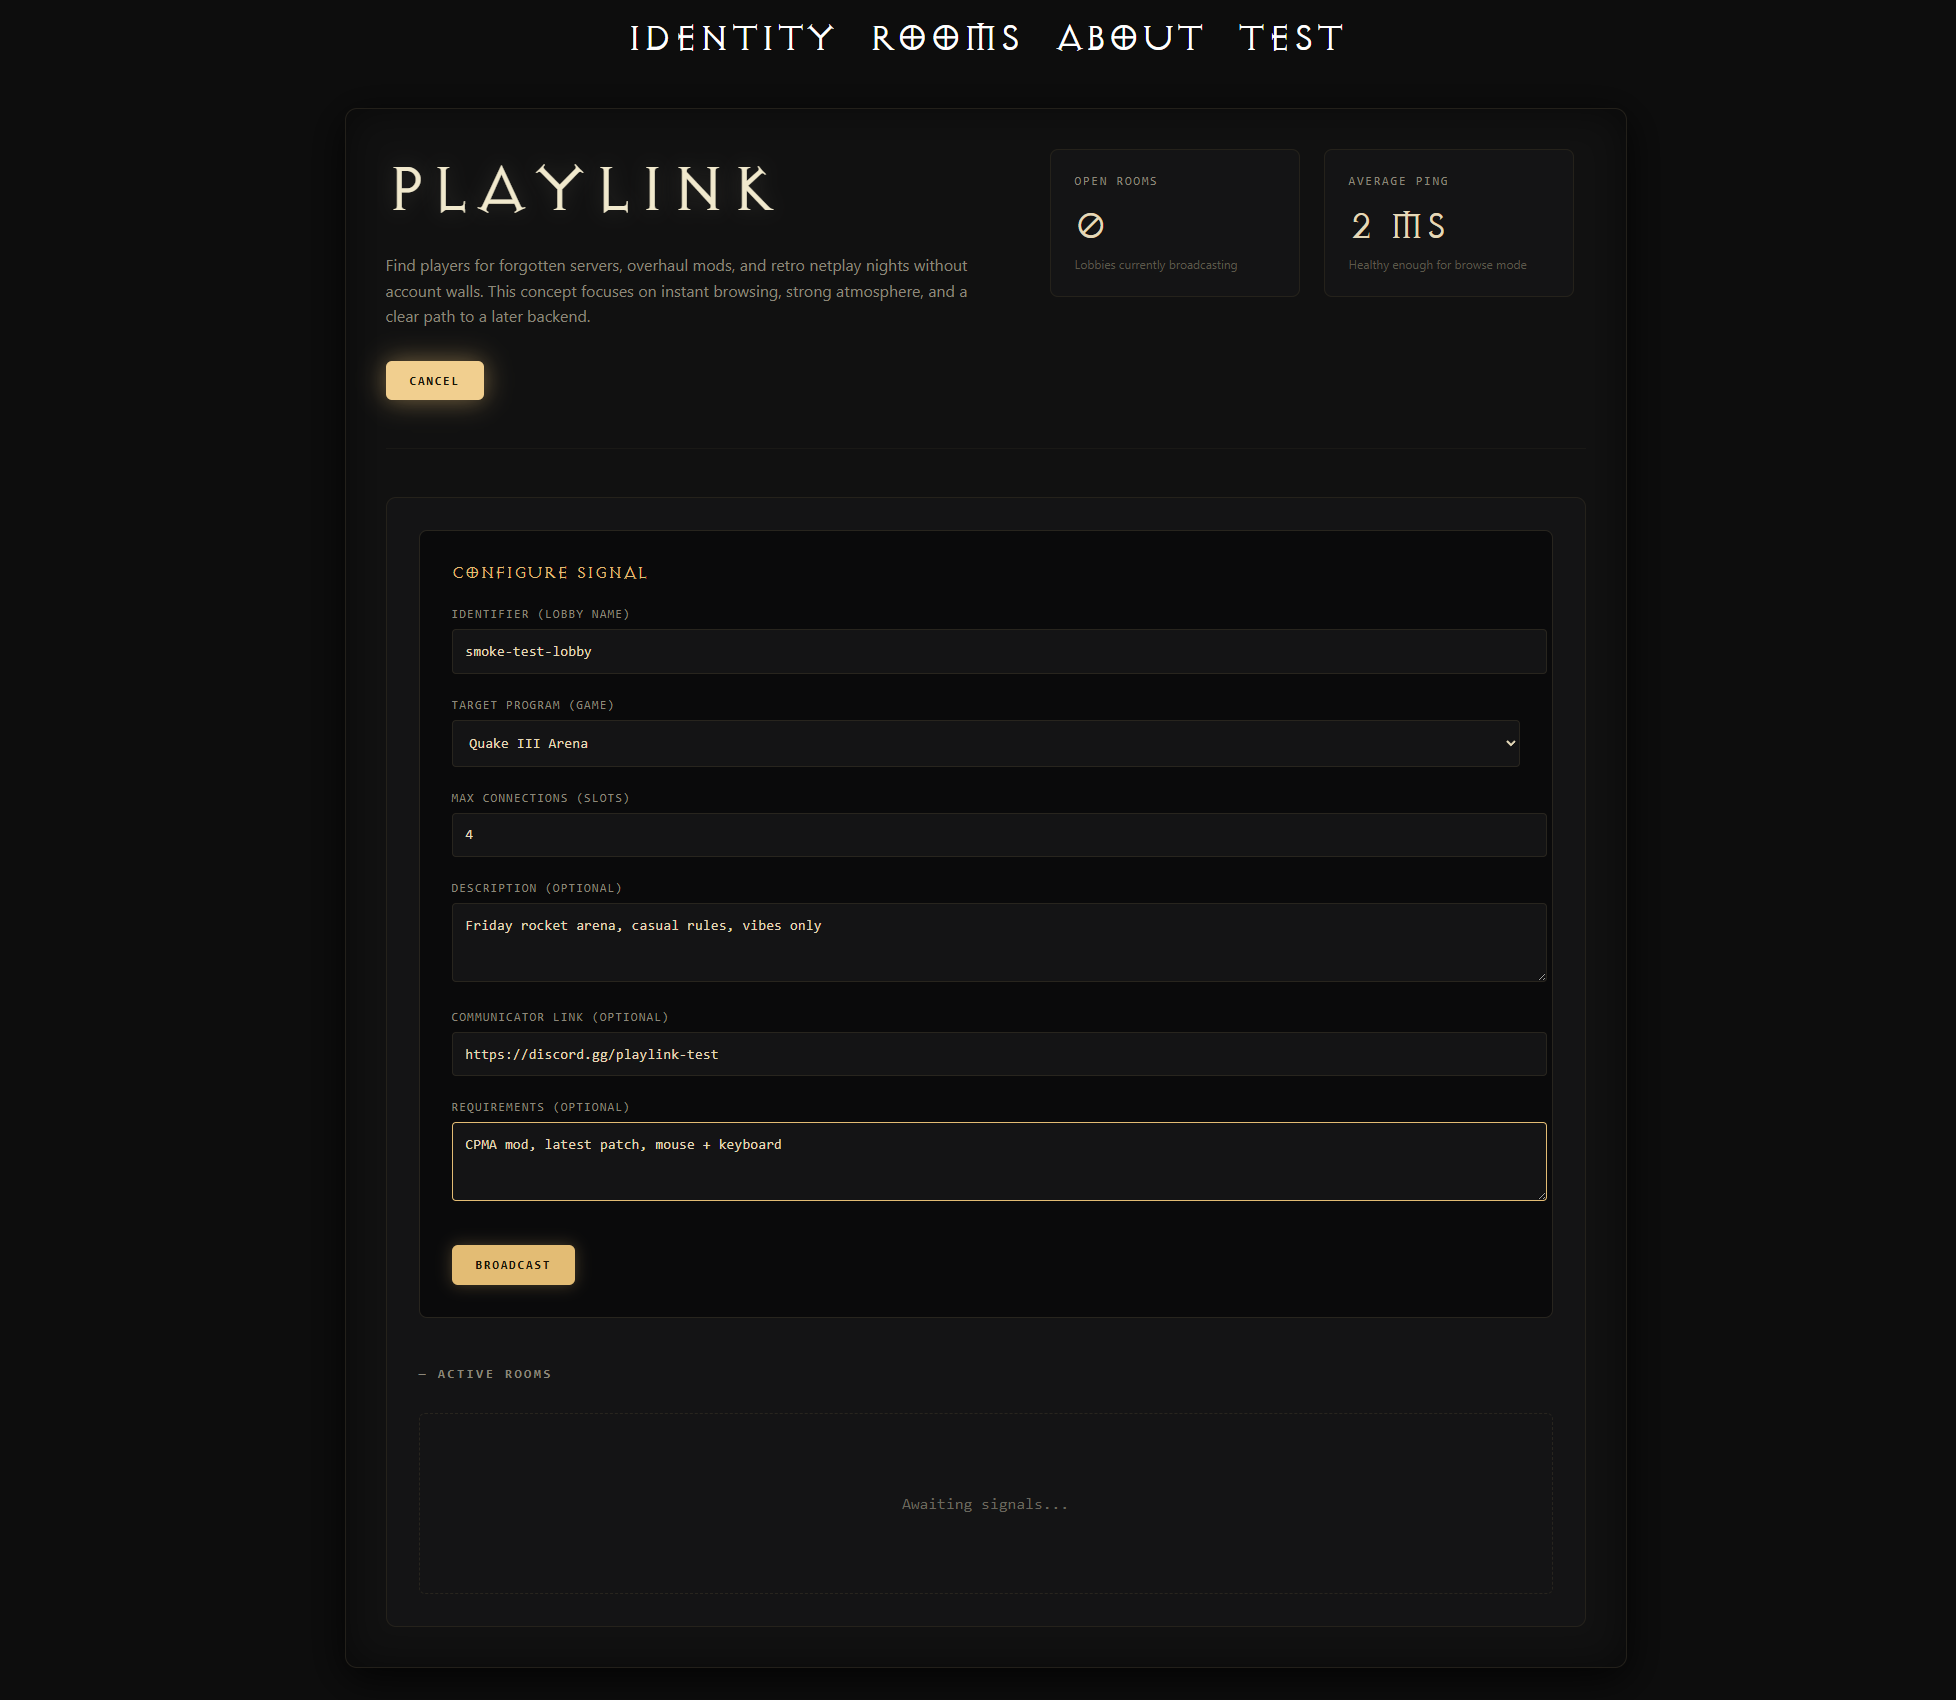
\includegraphics[width=\textwidth]{smoke-form-filled.png}
    \caption{Formularz tworzenia pokoju.}
  \end{subfigure}\hfill
  \begin{subfigure}[t]{0.48\textwidth}
    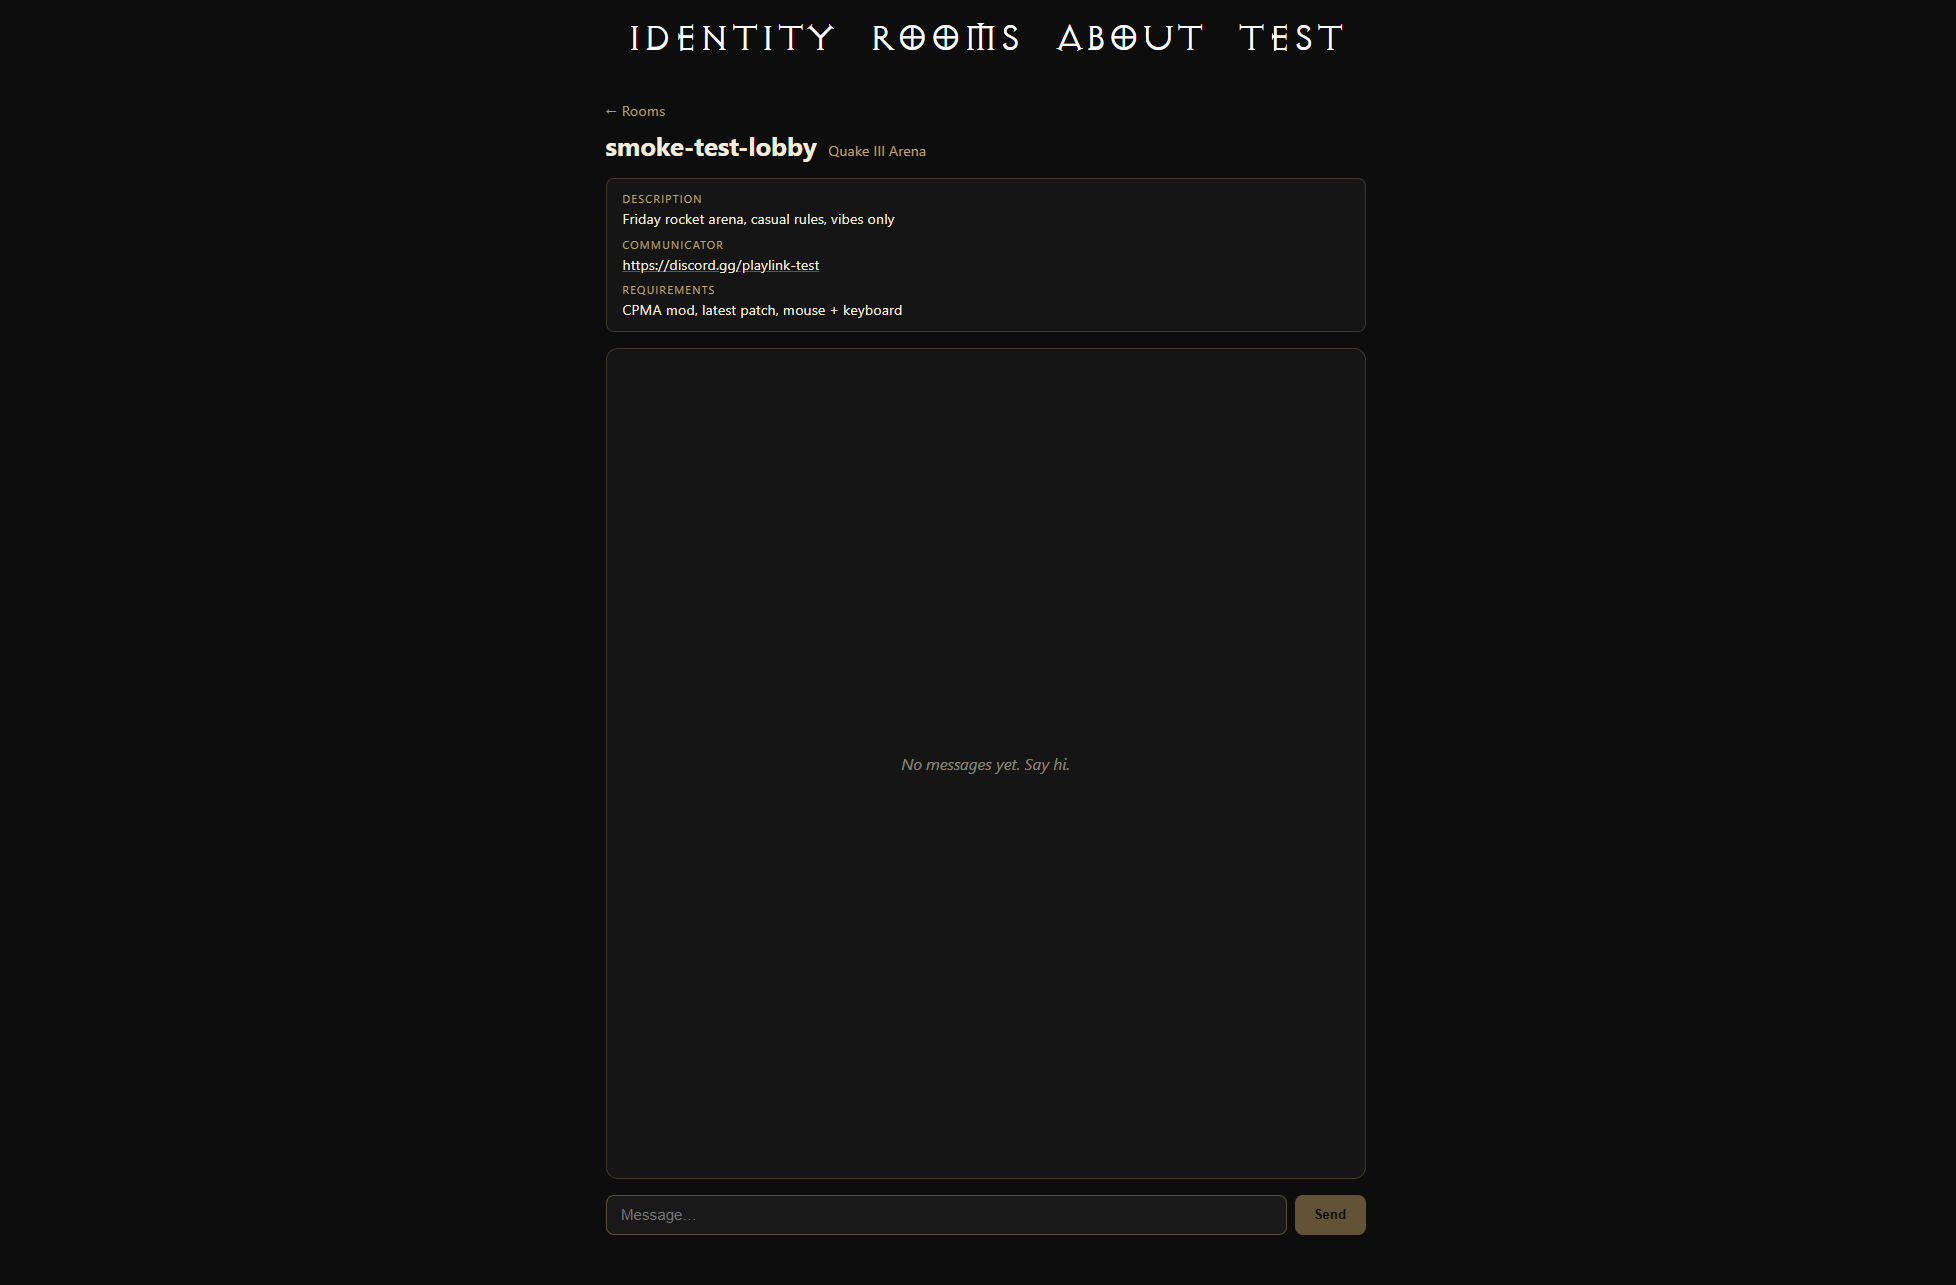
\includegraphics[width=\textwidth]{smoke-detail-with-metadata.png}
    \caption{Szczegóły pokoju z metadanymi.}
  \end{subfigure}

  \vspace{0.7em}
  \begin{subfigure}[t]{0.48\textwidth}
    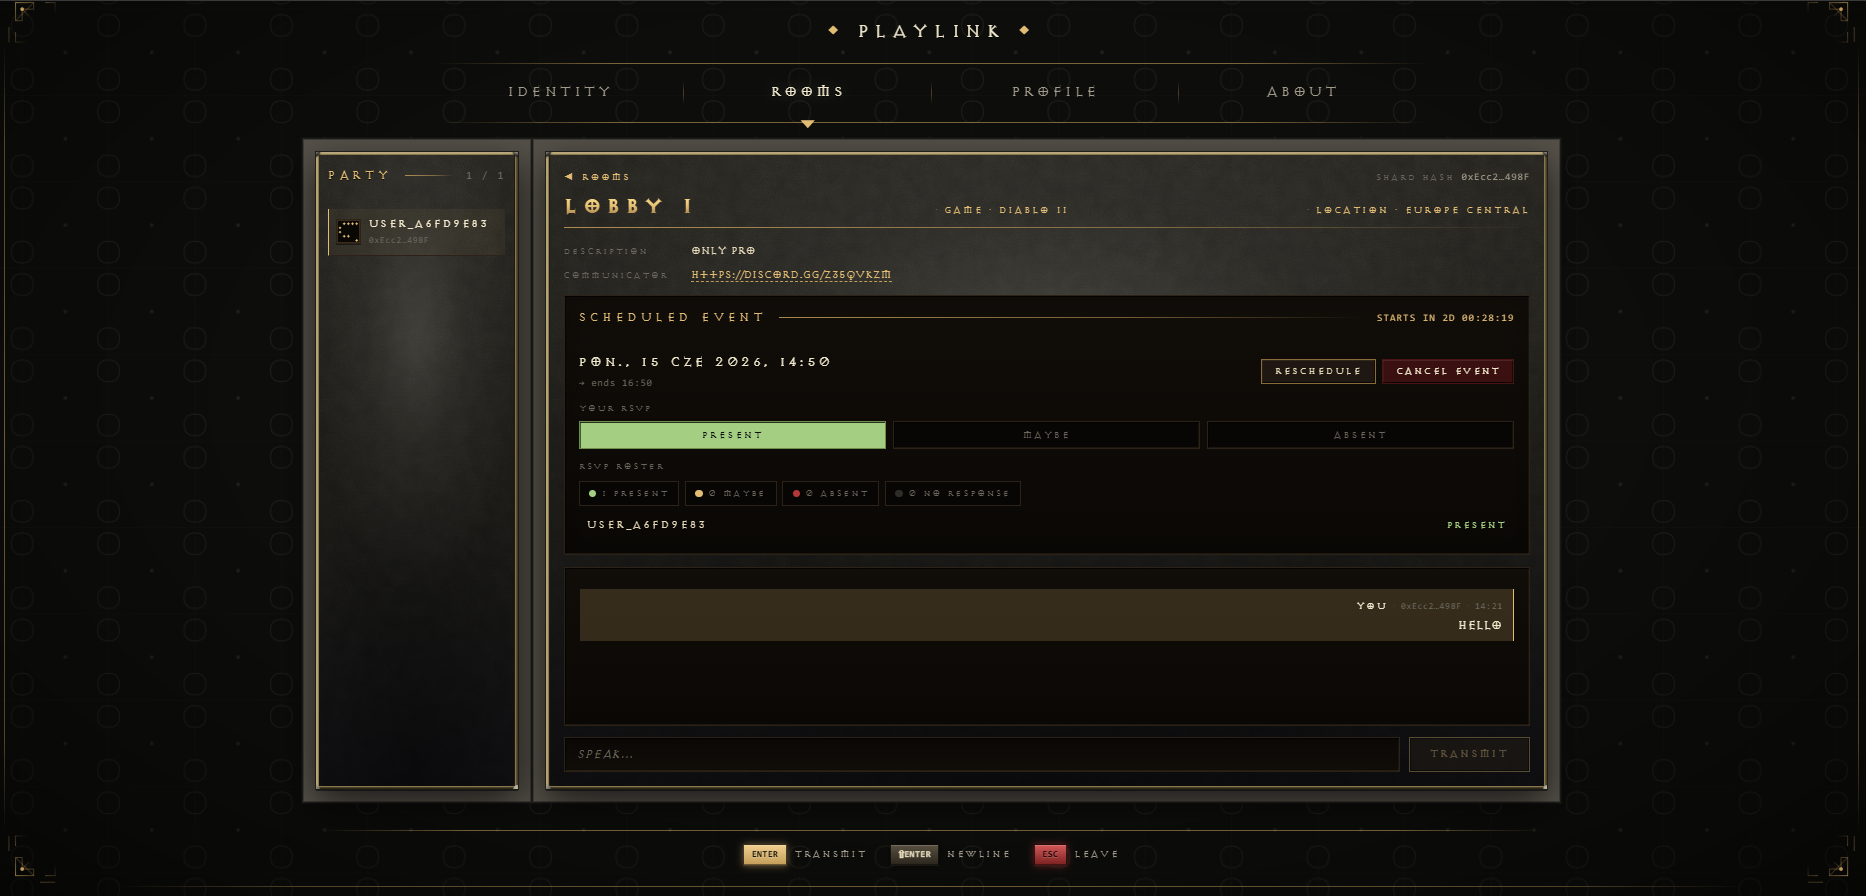
\includegraphics[width=\textwidth]{prez-slide29.png}
    \caption{Widok pokoju: uczestnicy, wydarzenie z RSVP, czat.}
  \end{subfigure}\hfill
  \begin{subfigure}[t]{0.48\textwidth}
    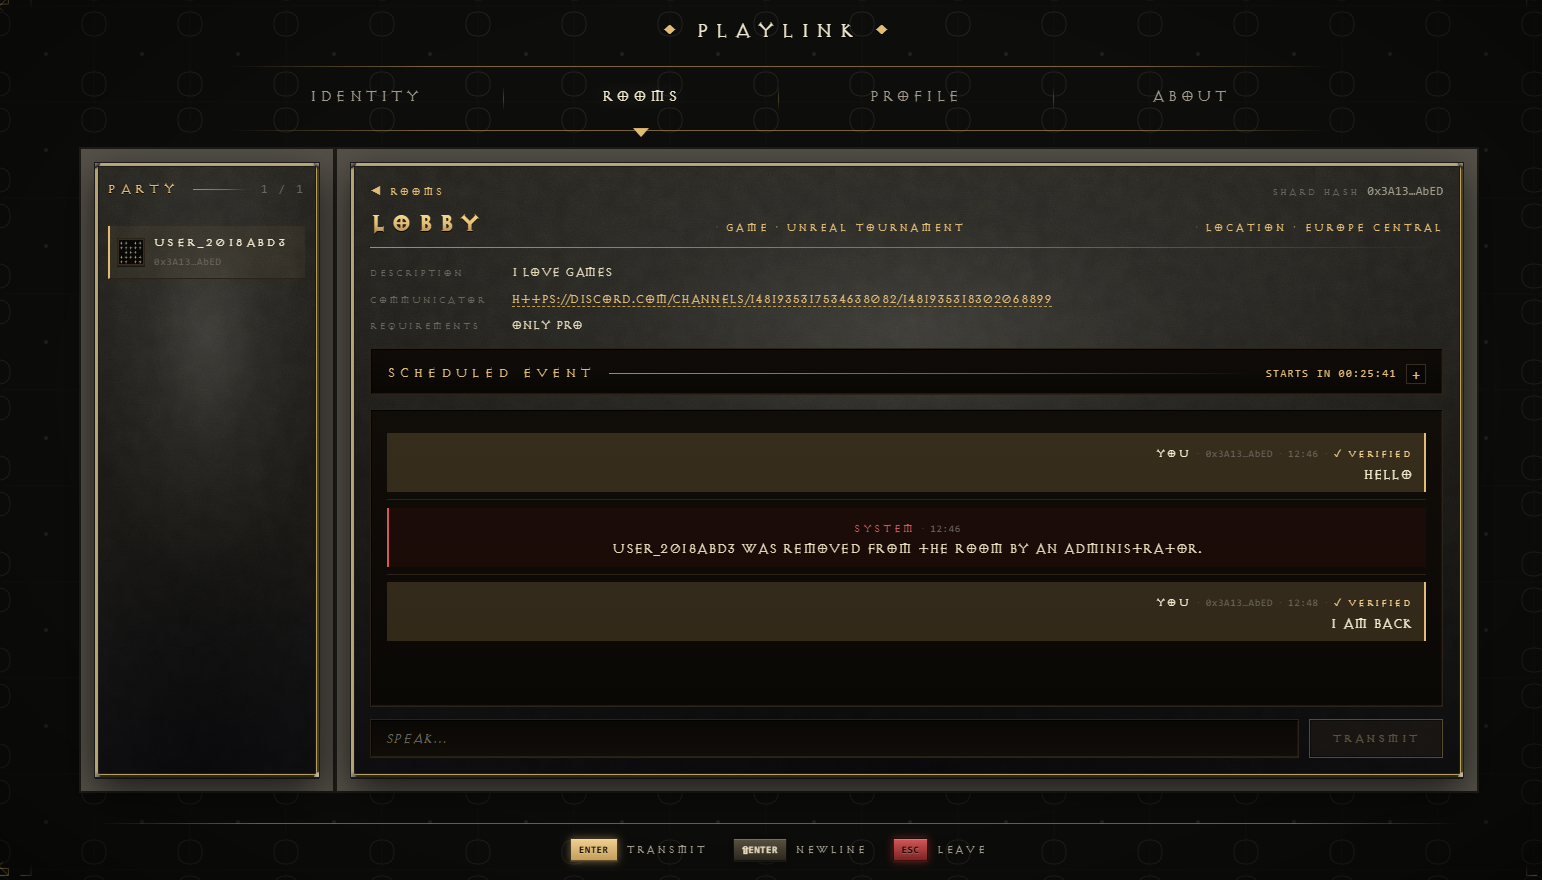
\includegraphics[width=\textwidth]{prez-slide35.png}
    \caption{Moderacja: zdarzenie systemowe o wyrzuceniu uczestnika.}
  \end{subfigure}
  \caption{Wybrane widoki graficznego interfejsu PlayLink.}
  \label{fig:gui}
\end{figure}

\subsection{Aspekty AI/ML}
\label{sec:aiml}

W uzgodnieniu z opiekunem projektu (mgr inż. Bartłomiej Jencz) zespół świadomie
zrezygnował z komponentu AI/ML na rzecz \textbf{rozszerzonego, dopracowanego modelu
bezpieczeństwa danych} (rozdz.~\ref{sec:bezp}). Decyzja wynika z charakteru produktu:
kluczową wartością PlayLink jest natychmiastowy, bezpieczny i prywatny dostęp
(tożsamość niepowiernicza BIP39, weryfikowalne autorstwo wiadomości), a nie
rekomendacje oparte na uczeniu maszynowym. Dobór pingu odbywa się deterministycznie
na podstawie odległości geograficznej lobby (metryka Haversine), bez modelu ML.

\subsection{Aspekty bezpieczeństwa danych}
\label{sec:bezp}

Bezpieczeństwo jest centralnym filarem PlayLink. Przyjęto zasadę \emph{non-custodial}:
klucz prywatny nigdy nie opuszcza przeglądarki, a backend wyłącznie weryfikuje dowody
kryptograficzne. Poniżej uzgodnione aspekty bezpieczeństwa — wszystkie zrealizowane
(pokrycie $\geq$90\%).

\paragraph{1. Tożsamość bezhasłowa (BIP39 + ECDSA).}
Konto reprezentuje 12-słowna fraza mnemoniczna BIP39 (standard z Bitcoina, 2013;
2048-wyrazowy słownik daje 132 bity entropii). Z frazy derywowany jest klucz
secp256k1, a publiczny adres EIP-55 stanowi identyfikator konta. Eliminuje to e-mail,
numer telefonu i hasło — a tym samym wektor ataku „reset hasła”.

\paragraph{2. Uwierzytelnianie challenge-response i ochrona przed replay.}
Logowanie wykorzystuje jednorazowy \emph{nonce}: backend wydaje wyzwanie, klient
podpisuje je (EIP-191 \code{personal_sign}), a backend odtwarza adres z podpisu
(ECDSA recovery). Zabezpieczenia:
\begin{itemize}
  \item nonce jest \textbf{jednorazowy} (flaga \code{used}) i \textbf{krótkożyciowy} (TTL 5~min);
  \item w bazie przechowywany jest wyłącznie \textbf{skrót SHA-256} wartości nonce —
        surowa wartość nigdy nie trafia na dysk;
  \item ponowne wydanie nonce unieważnia poprzedni — co blokuje ataki powtórzeniowe.
\end{itemize}

\paragraph{3. Izolacja tokenu sesji (wzorzec BFF, hardening XSS).}
Token JWT (HS256) jest przechowywany w ciasteczku \code{httpOnly},
\code{sameSite=strict}, ustawianym przez serwer SvelteKit. Token \textbf{nigdy nie jest
dostępny dla JavaScriptu klienta}, co znacząco ogranicza skutki ewentualnego XSS.

\paragraph{4. Weryfikowalne autorstwo wiadomości.}
Wiadomości czatu są podpisywane kluczem derywowanym z BIP39 (EIP-191). Serwer
rekonstruuje kanoniczną postać wiadomości i weryfikuje podpis, a znaczniki czasu
dryfujące ponad \code{CHAT_SIGNATURE_SKEW_SECONDS} są odrzucane — co ogranicza
powtórzenia. Autorstwo jest weryfikowalne \emph{end-to-end}, a nie tylko na podstawie JWT.

\paragraph{5. Autoryzacja administratora bez eskalacji.}
Uprawnienia administratora wynikają wyłącznie z listy adresów w zmiennej środowiskowej
\code{ADMIN_ADDRESSES} — w bazie nie istnieje kolumna \code{is_admin}. Uniemożliwia to
eskalację uprawnień przez modyfikację danych; sfałszowane roszczenie o admina jest
odrzucane (zob.\ testy bezpieczeństwa, rozdz.~\ref{sec:testy}).

\paragraph{6. Ograniczanie nadużyć (rate limiting) i higiena treści.}
REST jest limitowany przez slowapi (domyślnie 10/min), a czat — przesuwnym oknem
per-adres. Edycja nazwy użytkownika przechodzi przez filtr wulgaryzmów (stoplist).

\paragraph{7. Bezpieczeństwo sieci i wdrożenia.}
Cały ruch szyfrowany jest TLS~1.3 (HTTPS + WSS, certyfikaty Let's Encrypt). Wdrożenie
jest self-hosted: transfer artefaktów odbywa się prywatnym kanałem przez Tailscale
(mesh VPN, WireGuard), publiczny SSH nie jest wystawiony (brak ataków brute-force na
port~22), a baza PostgreSQL nie ma mapowania portu na hosta.

\paragraph{Weryfikacja.}
Wszystkie powyższe mechanizmy są pokryte automatycznymi testami bezpieczeństwa
(replay nonce, wygasły nonce, sfałszowane roszczenie admina, zmanipulowane podpisy) —
zob.\ rozdz.~\ref{sec:testy}.

% =====================================================================
\section{Testowanie rozwiązania}
\label{sec:testy}

PlayLink jest pokryty obszernym, zautomatyzowanym zestawem testów:
\textbf{135 testów} po stronie backendu (pytest) oraz \textbf{61 testów} po
stronie frontendu (Vitest). Pod względem \emph{różnorodności} wyróżniono
\textbf{sześć różnych rodzajów testów} (powyżej wymaganego minimum pięciu),
zestawionych w tab.~\ref{tab:typy-testow}. W podrozdziale~\ref{sec:katalog} opisano
ponadto \textbf{dziesięć reprezentatywnych przypadków testowych} (po kilka na rodzaj)
wraz z celem, metodą i wynikiem.

Pełna, rozszerzona dokumentacja testowa stanowi
\hyperref[sec:zalaczniki]{Załącznik B}. Obejmuje strategię i środowisko testowe,
22 szczegółowe przypadki, wyniki pokrycia i testów wydajnościowych oraz fragmenty
kodu testów pochodzące bezpośrednio z repozytorium.

\paragraph{Uwaga terminologiczna (różnorodność vs.\ liczba).}
Kryterium oceny dotyczy \emph{rodzajów} (typów) testów — wymaganych jest 5 różnych.
Liczba opisanych przypadków (10) to inna oś: są to konkretne testy rozłożone na owe
rodzaje (np.\ 2 na rodzaj). Oba wymagania są zatem spełnione jednocześnie: 6 rodzajów
oraz 10 szczegółowo udokumentowanych przypadków.

\renewcommand{\arraystretch}{1.3}
\begin{table}[H]
\centering\small
\begin{tabularx}{\textwidth}{@{}p{0.21\textwidth}p{0.18\textwidth}Yc@{}}
\toprule
\textbf{Rodzaj testów} & \textbf{Narzędzie} & \textbf{Zakres} & \textbf{Liczba} \\
\midrule
Jednostkowe & pytest, Vitest & Funkcje pomocnicze, walidacja, store'y, metryka Haversine & $\sim$25 \\
Integracyjne / API & FastAPI TestClient & Endpointy REST przez całą aplikację (SQLite in-memory) & $\sim$54 \\
WebSocket / realtime & TestClient WS & Rozgłaszanie ramek czatu i zdarzeń (34 połączenia WS) & $\sim$45 \\
Bezpieczeństwa & pytest + eth\_account & Replay, wygasły nonce, fałszywy admin, podrobione podpisy & $\sim$10 \\
Migracji (smoke) & pytest + Alembic & Migracja do \code{head}, weryfikacja schematu; w CI round-trip na Postgresie & 1 (+CI) \\
Kontraktowe (frontend) & Vitest & Server-loadery i akcje SvelteKit (\code{+page.server.ts}) & $\sim$20 \\
\bottomrule
\end{tabularx}
\caption{Sześć rodzajów testów w projekcie PlayLink.}
\label{tab:typy-testow}
\end{table}

\subsection{Charakterystyka rodzajów testów}

\paragraph{Testy jednostkowe.} Weryfikują izolowaną logikę bez bazy i sieci: parsowanie
listy adresów administratorów, funkcję \code{hash_nonce}, walidację nazw użytkownika,
a we frontendzie — podpisywanie, store'y oraz obliczanie odległości lobby (Haversine).
Narzędzia: pytest, Vitest + jsdom.

\paragraph{Testy integracyjne / API.} Uruchamiają żądania HTTP przez całą aplikację
FastAPI z użyciem \code{TestClient} i bazy SQLite in-memory (fixture nadpisuje
\code{get_session}). Pokrywają uwierzytelnianie, pełny cykl życia pokoju, panel
administratora i akcję kick — sprawdzając kody statusu oraz stan w bazie.

\paragraph{Testy WebSocket / realtime.} Wykorzystują \code{TestClient.websocket_connect}
(34 połączenia WS) do weryfikacji rozgłaszania ramek: \emph{event-update},
\emph{rsvp\_update}, \emph{roster\_update}, \emph{room\_closed}, \emph{member\_kicked}.

\paragraph{Testy bezpieczeństwa.} Najważniejszy rodzaj dla profilu projektu —
scenariusze ataków (replay, wygasły nonce, eskalacja uprawnień, podrobione podpisy
EIP-191), z realnym podpisywaniem kluczem (\code{eth_account}).

\paragraph{Testy migracji (smoke).} Aplikują pełny łańcuch Alembic
(\code{alembic upgrade head}) i sprawdzają obecność wszystkich ośmiu tabel; w CI
powtarzane na realnym PostgreSQL z round-tripem downgrade/upgrade i \code{alembic check}.

\paragraph{Testy kontraktowe frontendu.} Importują server-loadery i akcje SvelteKit
z zamockowanymi \code{fetch}/\code{cookies}, weryfikując przekierowania, strażników
autoryzacji i walidację formularzy.

\subsection{Katalog wybranych przypadków testowych}
\label{sec:katalog}

Poniżej opisano dziesięć reprezentatywnych przypadków testowych w jednolitym formacie
(rodzaj, cel, metoda/narzędzie, dane/kroki, oczekiwany wynik, rezultat). Wszystkie
przechodzą pomyślnie w pipeline CI; zespół może dołączyć do każdego zrzut ekranu
z wynikiem (np.\ raport pytest/Vitest lub log CI).

\newcommand{\tc}[7]{%
  \par\vspace{0.5em}\noindent\textbf{#1}\par\nopagebreak\vspace{0.2em}
  \noindent\begin{tabular}{@{}>{\itshape}p{0.20\textwidth}p{0.74\textwidth}@{}}
  Rodzaj & #2 \\
  Cel & #3 \\
  Metoda / narzędzie & #4 \\
  Dane / kroki & #5 \\
  Oczekiwany wynik & #6 \\
  Rezultat & #7 \\
  \end{tabular}\par\vspace{0.3em}\noindent\rule{\textwidth}{0.4pt}}

\tc{TC-01: Parsowanie adresów administratorów}
{Jednostkowy}
{Sprawdzić poprawne wczytanie i normalizację listy adresów z \code{ADMIN_ADDRESSES}.}
{pytest (\code{test_helpers.py}, \code{_parse_admin_addresses}).}
{Wejście \code{" 0xABC , 0xdef "} (spacje, różna wielkość liter).}
{Zbiór znormalizowanych adresów małymi literami: \code{{0xabc, 0xdef}}.}
{PASS}

\tc{TC-02: Hashowanie wartości nonce}
{Jednostkowy}
{Zapewnić, że nonce jest deterministycznie hashowany (SHA-256) przed zapisem.}
{pytest (\code{hash_nonce}).}
{Ten sam nonce hashowany dwukrotnie oraz dwa różne nonce.}
{Identyczny skrót dla identycznego wejścia; różne skróty dla różnych wejść.}
{PASS}

\tc{TC-03: Obliczanie odległości lobby (Haversine)}
{Jednostkowy (frontend)}
{Zweryfikować dobór pingu na podstawie odległości geograficznej lobby.}
{Vitest (\code{lobbyLocations.test.ts}).}
{Pary współrzędnych o znanej odległości.}
{Odległość w granicach tolerancji; właściwy przedział pingu.}
{PASS}

\tc{TC-04: Pełny przepływ logowania (challenge-response)}
{Integracyjny / API}
{Zweryfikować ścieżkę request-nonce $\rightarrow$ verify $\rightarrow$ wydanie JWT.}
{FastAPI \code{TestClient} (\code{test_auth.py}), podpis \code{eth_account}.}
{\code{POST /auth/request-nonce}, podpis nonce, \code{POST /auth/verify}.}
{HTTP 200 oraz poprawny token JWT i nazwa użytkownika w odpowiedzi.}
{PASS}

\tc{TC-05: Cykl życia pokoju i limit aktywnych pokojów}
{Integracyjny / API}
{Sprawdzić tworzenie, dołączanie, opuszczanie oraz limit 3 aktywnych pokojów.}
{FastAPI \code{TestClient} (\code{test_rooms_lifecycle.py}).}
{Sekwencja create/join/leave; próba utworzenia 4.\ pokoju.}
{Operacje 1--3 kończą się sukcesem; 4.\ pokój odrzucony błędem walidacji.}
{PASS}

\tc{TC-06: Rozgłaszanie wiadomości i ramek w czacie}
{WebSocket / realtime}
{Potwierdzić, że klienci otrzymują aktualizacje w czasie rzeczywistym.}
{\code{TestClient.websocket_connect} (\code{test_chat.py}, \code{test_room_events.py}).}
{Dwa połączenia WS w jednym pokoju; wysłanie wiadomości i zmiana RSVP.}
{Obaj klienci otrzymują ramki \emph{message}, \emph{rsvp-update}, \emph{roster-update}.}
{PASS}

\tc{TC-07: Odrzucenie ataku powtórzeniowego (replay)}
{Bezpieczeństwa}
{Uniemożliwić ponowne użycie tego samego nonce.}
{pytest (\code{test_verify_signature_rejects_replayed_nonce}).}
{Poprawna weryfikacja, a następnie ponowna z tym samym nonce/podpisem.}
{Pierwsza weryfikacja: 200; druga: odrzucenie (nonce oznaczony jako użyty).}
{PASS}

\tc{TC-08: Brak eskalacji uprawnień administratora}
{Bezpieczeństwa}
{Sfałszowane roszczenie o rolę admina nie może dawać dostępu.}
{pytest (\code{test_forged_admin_claim_does_not_grant_admin_access}).}
{Token/żądanie konta spoza \code{ADMIN_ADDRESSES} próbuje akcji administracyjnej.}
{HTTP 403; operacja administracyjna nie zostaje wykonana.}
{PASS}

\tc{TC-09: Migracja schematu bazy (smoke)}
{Migracji}
{Zapewnić, że pełny łańcuch migracji buduje poprawny schemat.}
{pytest + Alembic (\code{test_migrations.py}); w CI na PostgreSQL.}
{\code{alembic upgrade head} na świeżej bazie; inspekcja schematu.}
{Obecnych wszystkie 8 tabel i kluczowe kolumny; brak dryfu (\code{alembic check}).}
{PASS}

\tc{TC-10: Strażnik autoryzacji trasy (frontend)}
{Kontraktowy (frontend)}
{Niezalogowany użytkownik nie ma dostępu do tras chronionych.}
{Vitest (\code{rooms.name.page.server.test.ts}), zamockowane \code{cookies}/\code{fetch}.}
{Wywołanie \code{load} bez ważnej sesji.}
{Przekierowanie HTTP 303 do \code{/rooms}; brak ujawnienia danych chronionych.}
{PASS}

\subsection{Dokumentacja procesu i automatyzacja (CI)}
Proces testowy jest opisany w repozytorium (\code{docs/operations/testing.md} — tabele
pokrycia per plik, opis fixture'ów i kanałów WS). Konfiguracja: \code{pyproject.toml}
(\code{[tool.pytest.ini_options]}, pytest-cov), \code{vite.config.js} (Vitest, jsdom,
coverage-v8). Pipeline GitHub Actions (\code{.github/workflows/cicd.yml}) uruchamia
zadania: \code{backend-lint}, \code{backend-test} (z bramką \code{--cov-fail-under=80}),
\code{backend-migrations}, \code{frontend-lint}, \code{frontend-test} (z pokryciem) oraz
\code{build-test}. Zielony wynik wszystkich testów jest warunkiem wdrożenia
(\code{deploy}) oraz scalenia PR do \code{main}, co stanowi ciągłą, weryfikowalną
dokumentację wyników testowania.

% =====================================================================
\section{Zarządzanie projektem}
\label{sec:zarz}

\subsection{Cele i zakres projektu}

\textbf{Cel.} Stworzenie aplikacji webowej PlayLink umożliwiającej szybkie tworzenie i
wyszukiwanie sesji do wspólnej gry w niszowe, retro oraz mniej popularne tytuły
multiplayer.

\textbf{Zakres.} Projekt obejmuje: interfejs użytkownika, backend obsługujący sesje i
komunikację w czasie rzeczywistym oraz funkcje tworzenia, przeglądania, dołączania i
opuszczania sesji, czat w obrębie pokoju, bezhasłowe uwierzytelnianie (BIP39),
kalendarz/RSVP, panel administratora oraz pełną automatyzację wdrożenia (CI/CD).

\textbf{Co osiągnięto.} Zrealizowano wszystkie zaplanowane wymagania funkcjonalne i
niefunkcjonalne; aplikacja działa na środowisku produkcyjnym, ze szczególnym
naciskiem na bezpieczeństwo danych.

\subsection{Podział ról i zadań w zespole}

\renewcommand{\arraystretch}{1.3}
\begin{table}[H]
\centering\small
\begin{tabularx}{\textwidth}{@{}llY@{}}
\toprule
\textbf{Osoba (nr indeksu)} & \textbf{Rola} & \textbf{Wykonywane zadania} \\
\midrule
Jakub Rusek (247774) & Backend \& DevOps & Architektura backendu, autoryzacja, automatyzacja CI/CD (GitHub Actions), strategia wdrożeń, stabilność i dostępność. \\
Nikodem Nowak (251598) & Backend Developer & Logika serwerowa, implementacja API, komunikacja realtime (WebSocket), zarządzanie sesjami i bazą danych. \\
Bartosz Kołaciński (251554) & Frontend Developer & Budowa interfejsu użytkownika (UI/UX), integracja frontendu z backendem. \\
Mateusz Kosowski (251558) & Solution Architect & Projektowanie architektury rozwiązania, spójność decyzji technicznych, koordynacja integracji komponentów. \\
Jakub Rosiak (251620) & QA \& Documentation & Scenariusze testowe, walidacja kluczowych funkcji MVP, utrzymanie dokumentacji projektowej. \\
\bottomrule
\end{tabularx}
\caption{Podział ról i zadań w zespole projektowym.}
\label{tab:role}
\end{table}

\subsection{Harmonogram realizacji i kamienie milowe}

Projekt realizowano w sześciu etapach. Zestawienie etapów wraz z terminami i kamieniami
milowymi przedstawia tab.~\ref{tab:harmonogram}.

\renewcommand{\arraystretch}{1.3}
\begin{longtable}{@{}cp{0.16\textwidth}p{0.40\textwidth}p{0.24\textwidth}@{}}
\caption{Harmonogram realizacji projektu z kamieniami milowymi.}\label{tab:harmonogram}\\
\toprule
\textbf{Etap} & \textbf{Termin} & \textbf{Zakres prac} & \textbf{Kamień milowy} \\
\midrule
\endfirsthead
\toprule
\textbf{Etap} & \textbf{Termin} & \textbf{Zakres prac} & \textbf{Kamień milowy} \\
\midrule
\endhead
1 & Tydzień 3 & Analiza i założenia: cele i zakres, analiza rozwiązań, wymagania, podział ról, harmonogram, porządek repozytorium. & Zakończenie dokumentacji wstępnej. \\
2 & Tygodnie 4–5 & Projektowanie: architektura, struktura frontendu i backendu, główne widoki (user flow), lista zadań w Issues. & Gotowość do implementacji. \\
3 & Tygodnie 6–8 & Implementacja MVP: lista i tworzenie sesji, logika dołączania/opuszczania, integracja frontend–backend. & Działające MVP. \\
4 & Tygodnie 9–10 & Rozszerzenia i realtime: czat, WebSocket, dynamiczna aktualizacja listy pokojów. & Pełna wersja funkcjonalna. \\
5 & Do pocz.\ czerwca & Testy i poprawki: scenariusze użytkownika, walidacja formularzy, poprawki UI i stabilności, dokumentacja. & Gotowość na termin wstępny. \\
6 & Pocz.–poł.\ czerwca & Finalizacja: ostatnie poprawki, domknięcie zadań, wersja końcowa, przygotowanie do prezentacji. & Oddanie wersji końcowej. \\
\bottomrule
\end{longtable}

\paragraph{Podsumowanie kamieni milowych.}
(1)~Tydzień~3 — dokumentacja wstępna; (2)~Tydzień~5 — projekt rozwiązania;
(3)~Tydzień~8 — MVP; (4)~Tydzień~10 — pełna wersja funkcjonalna;
(5)~początek czerwca — gotowość na termin wstępny; (6)~połowa czerwca — wersja końcowa.

\subsection{Szczegółowy harmonogram: kluczowe wskaźniki efektywności (KPI)}

Dla każdego etapu zdefiniowano mierzalne KPI; zestawienie globalne przedstawia
tab.~\ref{tab:kpi}.

\renewcommand{\arraystretch}{1.3}
\begin{table}[H]
\centering\small
\begin{tabularx}{\textwidth}{@{}Yc@{}}
\toprule
\textbf{Wskaźnik (KPI)} & \textbf{Cel} \\
\midrule
Liczba przeanalizowanych rozwiązań konkurencyjnych & $\geq$ 3 \\
Liczba wymagań funkcjonalnych & $\geq$ 10 \\
Liczba wymagań niefunkcjonalnych & $\geq$ 5 \\
Procent ukończonych funkcji MVP (etap 4) & $\geq$ 90\% \\
Liczba działających funkcji realtime & $\geq$ 3 \\
Czas aktualizacji danych (realtime) & $<$ 1000~ms \\
Pokrycie testami backendu (bramka CI) & $\geq$ 80\% \\
Liczba otwartych błędów krytycznych przed oddaniem & 0 \\
Procent zamkniętych zadań (Issues) do połowy czerwca & $\geq$ 95\% \\
Czas wdrożenia (od \code{push} do live) & $\approx$ 3~min \\
\bottomrule
\end{tabularx}
\caption{Globalne kluczowe wskaźniki efektywności (KPI) projektu.}
\label{tab:kpi}
\end{table}

\paragraph{Wybrane KPI etapowe.}
\begin{itemize}
  \item \textbf{Etap 2:} architektura systemu 100\%; liczba opisanych głównych widoków
        $\geq$~4; liczba zadań implementacyjnych $\geq$~10.
  \item \textbf{Etap 3:} ukończone funkcje podstawowe $\geq$~70\%; zamknięte Issues
        $\geq$~60\% zaplanowanych; liczba błędów krytycznych $\leq$~5.
  \item \textbf{Etap 5:} przetestowane główne funkcje $\geq$~90\%; otwarte błędy
        krytyczne~0; czas reakcji na zgłoszony błąd $\leq$~2~dni.
  \item \textbf{Etap 6:} ukończone zadania projektowe $\geq$~95\%; otwarte zadania
        wysokiego priorytetu $\leq$~2.
\end{itemize}

\subsection{Narzędzia i proces pracy zespołowej}

Pracę zorganizowano w oparciu o GitHub: \textbf{Issues} (planowanie i podział zadań),
\textbf{Projects} z tablicą \textbf{Kanban} (przepływ \emph{Todo} $\rightarrow$
\emph{Awaiting Review} $\rightarrow$ \emph{Done}) oraz \textbf{Milestones} (kamienie
milowe). Obowiązywały zasady współpracy (\code{CONTRIBUTING.md}): rozwój na gałęziach
funkcyjnych, obowiązkowy przegląd Pull Requestów oraz konwencja komunikatów commitów.
Każdy PR musiał przejść zielony pipeline CI (lint + testy + build) przed scaleniem do
\code{main}, co zapewniało ciągłą jakość i czytelność dokumentacji projektowej.

% =====================================================================
\section{Załączniki}
\label{sec:zalaczniki}

Zgodnie z ustaleniami z prowadzącym niniejszy raport końcowy stanowi dokumentację
projektu. Poniższe materiały uzupełniające dołączono jako osobne pliki:

\begin{itemize}
  \item \textbf{Załącznik A — Dokumentacja techniczna}
        (\href{run:dokumentacja-techniczna.pdf}{\texttt{otwórz PDF}}:
        \bpath{dokumentacja-techniczna.pdf}): szczegółowy, deweloperski opis
        architektury, pełnego API REST, protokołu WebSocket, modelu danych,
        konfiguracji, migracji oraz wdrożenia — scalone materiały z katalogu
        \texttt{docs/} repozytorium.
  \item \textbf{Załącznik B — Dokumentacja testowa PlayLink}
        (\href{run:dokumentacja-testowa-playlink.pdf}{\texttt{otwórz PDF}}:
        \bpath{dokumentacja-testowa-playlink.pdf}): rozszerzona dokumentacja
        obejmująca strategię i środowisko testowe, wyniki wykonania zestawów,
        22 szczegółowe przypadki testowe, pomiary wydajności oraz przykładowe
        fragmenty kodu testów i konfiguracji CI.
\end{itemize}


\end{document}
